\documentclass[12pt,twoside,letterpaper]{article}
%NOTE: This report format is 
\setlength{\footskip}{1.5cm}

\newcommand{\reporttitle}{Procesadores de Lenguajes: Memoria del Proyecto}
\newcommand{\reportauthorOne}{Jose Luis Prado Sierra }
\newcommand{\cidOne}{220070}
\newcommand{\reportauthorTwo}{Alejandro Gragera Serradilla }
\newcommand{\cidTwo}{22M043}
\newcommand{\reportauthorThree}{Antonio Bielza Díez }
\newcommand{\cidThree}{22M049}
\newcommand{\reporttype}{Coursework}

% include files that load packages and define macros
\input{includes} % various packages needed for maths etc.
\input{notation} % short-hand notation and macros


%%%%%%%%%%%%%%%%%%%%%%%%%%%%

\raggedbottom
\begin{document}
% front page
% Last modification: 2016-09-29 (Marc Deisenroth)
% Modification for UW: 2017-05-22 (jphickey)
\begin{titlepage}

\newcommand{\HRule}{\rule{\linewidth}{0.5mm}} % Defines a new command for the horizontal lines, change thickness here


%----------------------------------------------------------------------------------------
%	LOGO SECTION
%----------------------------------------------------------------------------------------



\begin{center} % Center remainder of the page

%----------------------------------------------------------------------------------------
%	HEADING SECTIONS
%----------------------------------------------------------------------------------------

\includegraphics[width = 9cm]{./figures/etsiinf}\\[1.5cm] 
%\textbf{\textsc{\Large Procesadores de Lenguajes}}\\[1.0cm] 
\textsc{\Large Universidad Politécnica de Madrid}\\[0.5cm] 

%----------------------------------------------------------------------------------------
%	TITLE SECTION
%----------------------------------------------------------------------------------------
\vspace{0.75cm}
\HRule \\[0.4cm]
{ \huge \bfseries \reporttitle}\\ % Title of your document
\HRule \\[0.7cm]
    \textsc{\large Analizador Léxico y Tabla de Símbolos}
\end{center}
%----------------------------------------------------------------------------------------
%	AUTHOR SECTION
%----------------------------------------------------------------------------------------

%\begin{minipage}{0.4\hsize}
\vfill
\begin{flushright} \large
    \textsc{\textbf{Grupo 18}}
\\
\reportauthorOne - \cidOne\\ % Your name
\reportauthorTwo - \cidTwo\\ % Your name
\reportauthorThree - \cidThree\\ % Your name
\end{flushright}
%\vspace{4cm}
%\makeatletter
%Date: \@date 

%\vfill % Fill the rest of the page with whitespace



\makeatother


\end{titlepage}




%%%%%%%%%%%%%%%%%%%%%%%%%%% table of content
%If a table of content is needed, simply uncomment the following lines
\tableofcontents
\newpage

%%%%%%%%%%%%%%%%%%%%%%%%%%%% Main document
%\section*{Note:}
%\emph{This document is intended to provide a sample structure for the reports in ME303 at the University of Waterloo. }
\section{Introducción}
El objetivo de este proyecto es desarrollar un procesador de lenguajes capaz de reconocer y analizar un lenguaje de programación sencillo llamado MyJS, que es una versión reducida de JavaScript.\\ El procesador de lenguajes constará de tres componentes principales: un analizador léxico, un analizador sintáctico y un analizador semántico. Cada uno de estos componentes desempeñará un papel crucial en la comprensión y procesamiento del lenguaje MyJS.\\

En las siguientes secciones, se describirá en detalle el diseño y la implementación de cada uno de estos componentes, así como los desafíos enfrentados y las soluciones adoptadas durante el desarrollo del proyecto.\\

Para el uso del procesador de lenguajes, se tiene que ejecutar el siguiente comando en la terminal:
\begin{verbatim}
    python3 lex.py archivo_entrada.txt
\end{verbatim}

O desde el ejecutable con:
\begin{verbatim}
    ./myjs_analizer.exe archivo_entrada.txt
\end{verbatim}

\section{Analizador Léxico}
%\emph{Describe the physical problem under investigation and the briefly summarize the governing equations. Example:}

Durante el desarrollo del Analizador Léxico hemos descrito una serie de objetos y estructuras matemáticas indispensables para que su diseño, desarrollo y función final cumplan con las expectativas de un Procesador de Lenguajes.

\subsection{Tokens}

Los tokens son duplas que se generan cuando el Analizador Léxico encuentra una concatenación de caracteres que identifica como válida. 
\\
Contienen la información necesaria para que las reciba el Analizador Sintáctico y se componen de un código que los identifica y un atributo opcional que puede servir para diferenciarlos de otros tokens con el mismo código o aportar información extra.
\\
\\
Hemos definido los siguientes tokens en funcion de las necesidades de nuestra práctica:

\begin{itemize}[itemsep=0.1em, topsep=1em, parsep=0pt, partopsep=0pt]
    \item Boolean: $<$BOOLEAN, $>$
    \item Else: $<$ELSE, $>$
    \item Float: $<$FLOAT, $>$
    \item Function: $<$FUNCTION, $>$
    \item If: $<$IF, $>$
    \item Int: $<$INT, $>$
    \item Let: $<$LET, $>$
    \item Read: $<$READ, $>$
    \item Return: $<$RETURN, $>$
    \item String: $<$STRING, $>$
    \item Void: $<$VOID, $>$
    \item Write: $<$WRITE, $>$
    \item Constante real: $<$FLOATCONST, $>$
    \item Constante entera: $<$INTCONST, $>$
    \item Cadena: $<$STR, '$\text{c*}$'$>$
    \item Identificador: $<$ID, posTS$>$
    \item Suma con asignación [+=]: $<$PLUSEQ, $>$
    \item Igual [=]: $<$EQ, $>$
    \item Coma [,]: $<$COMMA, $>$
    \item Punto y coma [;]: $<$SEMICOLON, $>$
    \item Paréntesis abierto [(]: $<$OPPAR, $>$
    \item Paréntesis cerrado [)]: $<$CLPAR, $>$
    \item Llave abierta [\{]: $<$OPBRA, $>$
    \item Llave cerrada [\}]: $<$CLBRA, $>$
    \item Suma [+]: $<$SUM, $>$
    \item Y Lógico [\&\&]: $<$AND, $>$
    \item Menor [$<$]: $<$MINORTHAN, $>$
    \item false: $<$FALSE, $>$
    \item true: $<$TRUE, $>$
    \item EOF: $<$EOF, $>$
\end{itemize}

Todos los tokens anteriores conforman todos los obligatorios, los específicos y los opcionales de la práctica.

\subsection{Gramática}

La gramática es la estructura matemática que define el lenguaje a generar, en nuestros caso es para una versión reducida de JS. Definir la gramática es una forma de estructurar por tanto el lenguaje y asegurarnos de que vamos a generar solo lo que queremos.
\\
\\
Hemos definido las siguientes reglas:
\begin{itemize}[label={}, itemsep=0.0em, topsep=0.5em]
    \item $S \to ~delS~|~+A~|~\&B~|~`C~|~dD~|~lF~|~\_F~|~/G~|~=~|~,~|~;~|~<~|~(~|~)~|~\{~|~\}$
    \item $A \to ~=~|~\lambda$
    \item $B \to ~\&$
    \item $C \to ~cC~|~`$
    \item $D \to ~dD~|~.E~|~\lambda$
    \item $E \to ~dE~|~d$
    \item $F \to ~lF~|~dF~|~\_F~|~\lambda$
    \item $G \to ~/H$
    \item $H \to ~c_2H~|~\text{\textbackslash n}S$
\end{itemize}
\vspace{1em}
Los conjuntos definidos para el desarrollo de la gramática y del resto de la práctica son: 
\begin{itemize}[label={}, itemsep=0.0em, topsep=0.5em]
    \item Conjunto l: representa cualquier letra.
    \item Conjunto d: representa cualquier dígito.
    \item Conjunto c: representa cualquier caracter.
    \item Conjunto c$_2$: representa cualquier caracter sin \textbackslash n.
\end{itemize}

\subsection{Autómata}

Un autómata es otro tipo de estructura matemática capaz de, al contrario que una gramática que se centra en generar un lenguaje, este se encarga de comprenderlo.
\\
\\
El autómata que hemos planteado capaz de entender todas las palabras válidas de nuestro lenguaje es el siguiente:

\begin{center}
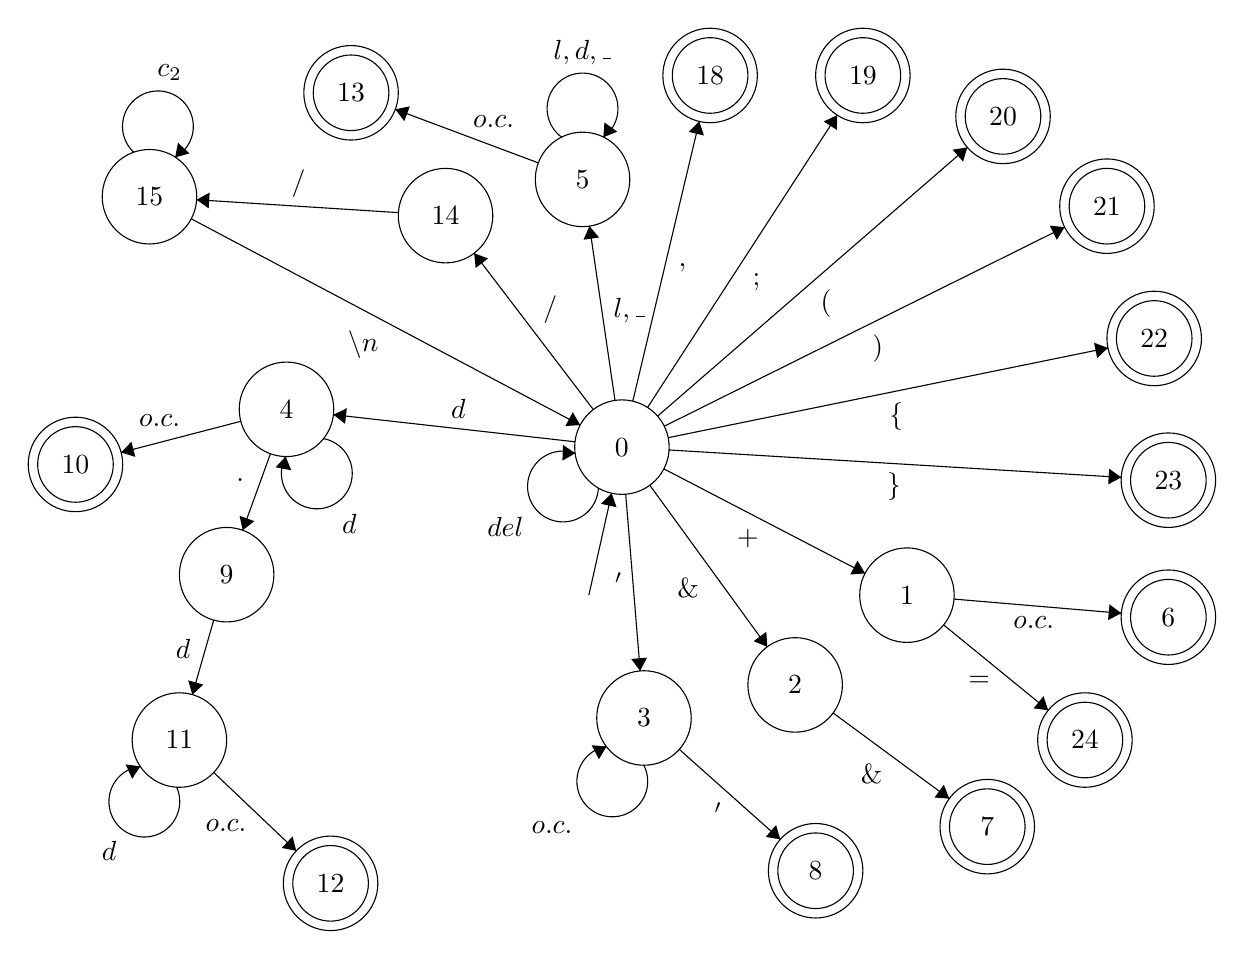
\begin{tikzpicture}[scale=0.2]
\tikzstyle{every node}+=[inner sep=0pt]
\draw [black] (39.8,-27.7) circle (3);
\draw (39.8,-27.7) node {$0$};
\draw [black] (57.9,-37.1) circle (3);
\draw (57.9,-37.1) node {$1$};
\draw [black] (74.5,-38.5) circle (3);
\draw (74.5,-38.5) node {$6$};
\draw [black] (74.5,-38.5) circle (2.4);
\draw [black] (69.2,-46.3) circle (3);
\draw (69.2,-46.3) node {$24$};
\draw [black] (69.2,-46.3) circle (2.4);
\draw [black] (50.8,-42.8) circle (3);
\draw (50.8,-42.8) node {$2$};
\draw [black] (63,-51.8) circle (3);
\draw (63,-51.8) node {$7$};
\draw [black] (63,-51.8) circle (2.4);
\draw [black] (41.2,-44.9) circle (3);
\draw (41.2,-44.9) node {$3$};
\draw [black] (52.1,-54.6) circle (3);
\draw (52.1,-54.6) node {$8$};
\draw [black] (52.1,-54.6) circle (2.4);
\draw [black] (18.5,-25.3) circle (3);
\draw (18.5,-25.3) node {$4$};
\draw [black] (5.1,-28.8) circle (3);
\draw (5.1,-28.8) node {$10$};
\draw [black] (5.1,-28.8) circle (2.4);
\draw [black] (14.7,-35.8) circle (3);
\draw (14.7,-35.8) node {$9$};
\draw [black] (11.7,-46.3) circle (3);
\draw (11.7,-46.3) node {$11$};
\draw [black] (21.3,-55.4) circle (3);
\draw (21.3,-55.4) node {$12$};
\draw [black] (21.3,-55.4) circle (2.4);
\draw [black] (28.6,-13) circle (3);
\draw (28.6,-13) node {$14$};
\draw [black] (9.8,-11.8) circle (3);
\draw (9.8,-11.8) node {$15$};
\draw [black] (37.3,-10.7) circle (3);
\draw (37.3,-10.7) node {$5$};
\draw [black] (22.6,-5.2) circle (3);
\draw (22.6,-5.2) node {$13$};
\draw [black] (22.6,-5.2) circle (2.4);
\draw [black] (45.4,-4.1) circle (3);
\draw (45.4,-4.1) node {$18$};
\draw [black] (45.4,-4.1) circle (2.4);
\draw [black] (55.1,-4.1) circle (3);
\draw (55.1,-4.1) node {$19$};
\draw [black] (55.1,-4.1) circle (2.4);
\draw [black] (64,-6.7) circle (3);
\draw (64,-6.7) node {$20$};
\draw [black] (64,-6.7) circle (2.4);
\draw [black] (70.6,-12.4) circle (3);
\draw (70.6,-12.4) node {$21$};
\draw [black] (70.6,-12.4) circle (2.4);
\draw [black] (73.6,-20.8) circle (3);
\draw (73.6,-20.8) node {$22$};
\draw [black] (73.6,-20.8) circle (2.4);
\draw [black] (74.5,-29.8) circle (3);
\draw (74.5,-29.8) node {$23$};
\draw [black] (74.5,-29.8) circle (2.4);
\draw [black] (38.305,-30.288) arc (-2.28448:-290.28448:2.25);
\draw (33.58,-32.78) node [left] {$del$};
\fill [black] (36.84,-28.09) -- (36.06,-27.56) -- (36.02,-28.56);
\draw [black] (42.46,-29.08) -- (55.24,-35.72);
\fill [black] (55.24,-35.72) -- (54.76,-34.9) -- (54.3,-35.79);
\draw (47.8,-32.9) node [below] {$+$};
\draw [black] (60.23,-38.99) -- (66.87,-44.41);
\fill [black] (66.87,-44.41) -- (66.57,-43.51) -- (65.94,-44.29);
\draw (62.48,-42.19) node [below] {$=$};
\draw [black] (60.89,-37.35) -- (71.51,-38.25);
\fill [black] (71.51,-38.25) -- (70.76,-37.68) -- (70.67,-38.68);
\draw (65.95,-38.43) node [below] {$o.c.$};
\draw [black] (41.57,-30.12) -- (49.03,-40.38);
\fill [black] (49.03,-40.38) -- (48.97,-39.43) -- (48.16,-40.02);
\draw (44.72,-36.63) node [left] {$\&$};
\draw [black] (53.21,-44.58) -- (60.59,-50.02);
\fill [black] (60.59,-50.02) -- (60.24,-49.14) -- (59.65,-49.95);
\draw (55.65,-47.8) node [below] {$\&$};
\draw [black] (40.04,-30.69) -- (40.96,-41.91);
\fill [black] (40.96,-41.91) -- (41.39,-41.07) -- (40.39,-41.15);
\draw (39.88,-36.36) node [left] {$'$};
\draw [black] (41.184,-47.888) arc (27.43495:-260.56505:2.25);
\draw (35.36,-51.45) node [below] {$o.c.$};
\fill [black] (38.82,-46.71) -- (37.88,-46.63) -- (38.34,-47.52);
\draw [black] (43.44,-46.89) -- (49.86,-52.61);
\fill [black] (49.86,-52.61) -- (49.59,-51.7) -- (48.93,-52.45);
\draw (45.92,-50.24) node [below] {$'$};
\draw [black] (36.82,-27.36) -- (21.48,-25.64);
\fill [black] (21.48,-25.64) -- (22.22,-26.22) -- (22.33,-25.23);
\draw (29.41,-25.9) node [above] {$d$};
\draw [black] (20.842,-27.156) arc (79.34618:-208.65382:2.25);
\draw (22.49,-31.91) node [below] {$d$};
\fill [black] (18.45,-28.29) -- (17.81,-28.98) -- (18.8,-29.17);
\draw [black] (15.6,-26.06) -- (8,-28.04);
\fill [black] (8,-28.04) -- (8.9,-28.32) -- (8.65,-27.36);
\draw (10.44,-26.43) node [above] {$o.c.$};
\draw [black] (17.48,-28.12) -- (15.72,-32.98);
\fill [black] (15.72,-32.98) -- (16.46,-32.4) -- (15.52,-32.06);
\draw (15.84,-29.77) node [left] {$.$};
\draw [black] (13.88,-38.68) -- (12.52,-43.42);
\fill [black] (12.52,-43.42) -- (13.22,-42.78) -- (12.26,-42.51);
\draw (12.43,-40.49) node [left] {$d$};
\draw [black] (11.522,-49.283) arc (24.30891:-263.69109:2.25);
\draw (7.24,-52.67) node [below] {$d$};
\fill [black] (9.22,-47.97) -- (8.29,-47.85) -- (8.7,-48.76);
\draw [black] (13.88,-48.36) -- (19.12,-53.34);
\fill [black] (19.12,-53.34) -- (18.89,-52.42) -- (18.2,-53.15);
\draw (14.66,-51.33) node [below] {$o.c.$};
\draw [black] (37.98,-25.31) -- (30.42,-15.39);
\fill [black] (30.42,-15.39) -- (30.51,-16.33) -- (31.3,-15.72);
\draw (34.77,-18.95) node [right] {$/$};
\draw [black] (25.61,-12.81) -- (12.79,-11.99);
\fill [black] (12.79,-11.99) -- (13.56,-12.54) -- (13.62,-11.54);
\draw (19.26,-11.85) node [above] {$/$};
\draw [black] (8.806,-8.982) arc (227.15994:-60.84006:2.25);
\draw (11.08,-4.44) node [above] {$c_2$};
\fill [black] (11.43,-9.3) -- (12.34,-9.05) -- (11.61,-8.37);
\draw [black] (39.36,-24.73) -- (37.74,-13.67);
\fill [black] (37.74,-13.67) -- (37.36,-14.53) -- (38.35,-14.39);
\draw (39.24,-19.02) node [right] {$l,\_$};
\draw [black] (35.977,-8.02) arc (234:-54:2.25);
\draw (37.3,-3.45) node [above] {$l,d,\_$};
\fill [black] (38.62,-8.02) -- (39.5,-7.67) -- (38.69,-7.08);
\draw [black] (34.49,-9.65) -- (25.41,-6.25);
\fill [black] (25.41,-6.25) -- (25.98,-7) -- (26.33,-6.06);
\draw (31.65,-7.41) node [above] {$o.c.$};
\draw [black] (40.49,-24.78) -- (44.71,-7.02);
\fill [black] (44.71,-7.02) -- (44.04,-7.68) -- (45.01,-7.91);
\draw (43.36,-16.32) node [right] {$,$};
\draw [black] (41.43,-25.18) -- (53.47,-6.62);
\fill [black] (53.47,-6.62) -- (52.61,-7.02) -- (53.45,-7.56);
\draw (48.07,-17.22) node [right] {$;$};
\draw [black] (42.07,-25.73) -- (61.73,-8.67);
\fill [black] (61.73,-8.67) -- (60.8,-8.81) -- (61.46,-9.57);
\draw (52.76,-17.69) node [below] {$($};
\draw [black] (42.49,-26.37) -- (67.91,-13.73);
\fill [black] (67.91,-13.73) -- (66.97,-13.64) -- (67.42,-14.54);
\draw (56.04,-20.55) node [below] {$)$};
\draw [black] (42.74,-27.1) -- (70.66,-21.4);
\fill [black] (70.66,-21.4) -- (69.78,-21.07) -- (69.98,-22.05);
\draw (57.23,-24.83) node [below] {$\{$};
\draw [black] (42.79,-27.88) -- (71.51,-29.62);
\fill [black] (71.51,-29.62) -- (70.74,-29.07) -- (70.68,-30.07);
\draw (57.08,-29.3) node [below] {$\}$};
\draw [black] (37.7,-37.1) -- (39.15,-30.63);
\fill [black] (39.15,-30.63) -- (38.48,-31.3) -- (39.46,-31.52);
\draw [black] (12.45,-13.2) -- (37.15,-26.3);
\fill [black] (37.15,-26.3) -- (36.68,-25.48) -- (36.21,-26.36);
\draw (23.37,-20.25) node [below] {$\backslash n$};
\end{tikzpicture}
\end{center}

El autómata tiene que ir acompañado de una serie de acciones que realizar mientras se recorre para poder generar los tokens mientras vamos leyendo el archivo, que vamos a plantear en el siguiente punto.
\\
\\
Cuando aparece una transición o.c. significa que es cualquier otro caracter distinto a las demás transiciones salientes del vértice.

\subsection{Acciones Semánticas}

Las acciones semánticas son una serie de acciones que se realizan entre las transiciones del autómata que permiten realizar diferentes funciones como por ejemplo ir generando un string para cuando detectamos una cadena.
\\
\\
Las acciones semánticas que hemos definido para nuestro proyecto son:
\begin{itemize}[label={-}, itemsep=0.0em, topsep=0.5em]
    \item 0:0 Leer
    \item 0:18 Leer, gentoken($<$COMMA, $>$)
    \item 0:19 Leer, gentoken($<$SEMICOLON, $>$)
    \item 0:20 Leer, gentoken($<$OPPAR, $>$)
    \item 0:21 Leer, gentoken($<$CLPAR, $>$)
    \item 0:22 Leer, gentoken($<$OPBRA, $>$)
    \item 0:23 Leer, gentoken($<$CLBRA, $>$)
    \item 0:1 Leer
    \item 1:6 gentoken($<$SUM, $>$)
    \item 1:24 Leer, gentoken($<$EQ, $>$)
    \item 0:2 Leer
    \item 2:7 Leer, gentoken($<$AND, $>$)
    \item 0:3 Leer, $str=''$
    \item 3:3 Leer, $str=str + c$
    \item 3:8 Leer
        \subitem if (len(str) $>$ 64) error('Cadena demasiado larga')
        \subitem else gentoken($<$STRING, str$>$)
    \item 0:4 Leer, $num=d$
    \item 4:4 Leer, $num = num*10 + d$
    \item 4:10  
        \subitem if (num $>$ 32767) error('Entero demasiado grande')
        \subitem else gentoken($<$INTCONST, num$>$)
    \item 4:9 Leer, $cont=1$
    \item 9:11 Leer, $num = num*10 + d$, $cont++$
    \item 11:11 Leer, $num = num*10 + d$, $cont++$
    \item 11:12 $num = num*10^{-cont}$
        \subitem if (num $>$ 117549436) error('Real demasiado grande')
        \subitem else gentoken($<$FLOATCONST, num$>$)
    \item 0:14 Leer
    \item 0:15 Leer
    \item 15:15 Leer
    \item 15:0 Leer
    \item 0:5 Leer, $id=c$
    \item 5:5 Leer, $id=id + c$
    \item 5:13
        \subitem if (id in palabrasReservadas)
            gentoken($<$toUpper(id), $>$)
        \subitem else \{
            \subsubitem if( not inTS(id) ) 
                posTS = insertTS(id)
            \subsubitem gentoken($<$ID, posTS$>$)
        \subitem \}
    \vspace{-0.2cm}
\end{itemize}


\subsection{Errores}

Todo buen procesador de lenguajes debe de avisar al usuario de si existe algún error y además es capaz de tratar todos los posibles errores para una ejecución robusta y comprensible. 
\\
Sin embargo para esta entrega no es necesario que sean descriptivos pero si han de ser reconocidos y clasificados.
\\
\\
Hemos detectado los siguientes casos capaces de generar errores:
\begin{itemize}[itemsep=0.0em, topsep=0.5em]
    \item \textbf{Cadena mal cerrada:} Al iniciar una cadena si queda mal cerrada (Ej. 'Hola buenas tardes).
    \item \textbf{ID incorrecto:} Al generar o utilizar un ID si los caracteres que lo componen no son correctos.
    \item \textbf{Caracter no reconocido:} Si se recibe un caracter no válido en el estado inicial.
    \item \textbf{Operador lógico incorrecto:} Si se pone un operador lógico (como \&\&) de forma incorrecta (Ej. \&).
    \item \textbf{Comentario de línea mal iniciado:} Al iniciar un comentario de línea incorrectamente (Ej. /Hola buenas tardes).
    \item \textbf{Entero demasiado grande:} Al declarar un entero mayor que 32767.
    \item \textbf{Real demasiado grande:} Al declarar un real mayor que 117549436.
    \item \textbf{Cadena demasiado grande:} Al declarar una cadena de más de 64 caracteres.
\end{itemize}


\section{Analizador Sintáctico}

Durante el desarrollo del Analizador Sintáctico hemos descrito una gramática y desarrollado un programa que, junto al analizador léxico, es capaz de reconocer y analizar correctamente el lenguaje planteado para el desarrollo de la práctica.

\subsection{Gramática}

La gramática planteada para el desarrollo de Analizador Sintáctico es de tipo 2 segun la jerarquía de Chomsky, es decir, una gramática libre de contexto. Además cumple con las propiedades necesarias para ser LL(1), lo que nos permite desarrollar un analizador sintáctico predictivo.
\\\\
Teniendo todo lo anterior en cuenta, la gramática definida es la siguiente:

\begin{enumerate}[label=\textbf{\arabic*:}]
  \item \texttt{S} $\to$ \texttt{LC S | LF S | eof}
  \item \texttt{LC} $\to$ \texttt{LS semicolon | if oppar Expresion clpar CuerpoIf LE}
  \item \texttt{LE} $\to$ \texttt{else CuerpoIf |} $\lambda$
  \item \texttt{LF} $\to$ \texttt{function TypeFun id oppar Args clpar opbra Cuerpo clbra}
  \item \texttt{CuerpoIf} $\to$ \texttt{opbra Cuerpo clbra | LC}
  \item \texttt{Cuerpo} $\to$ \texttt{LC Cuerpo |} $\lambda$
  \item \texttt{Args} $\to$ \texttt{Tipo id ArgMore | void |} $\lambda$
  \item \texttt{ArgsLlamada} $\to$ \texttt{Expresion ArgMoreLlamada | void |} $\lambda$
  \item \texttt{ArgMoreLlamada} $\to$ \texttt{comma Expresion ArgMoreLlamada |} $\lambda$
  \item \texttt{ArgMore} $\to$ \texttt{comma Tipo id ArgMore |} $\lambda$
  \item \texttt{LS} $\to$ \texttt{let Tipo id Asignar | id IdOpt | read id | write Expresion | return ExpReturn}
  \item \texttt{IdOpt} $\to$ \texttt{oppar ArgsLlamada clpar | eq Expresion | pluseq Expresion}
  \item \texttt{TypeFun} $\to$ \texttt{void | Tipo}
  \item \texttt{Tipo} $\to$ \texttt{int | float | string | boolean}
  \item \texttt{Asignar} $\to$ \texttt{eq Expresion |} $\lambda$
  \item \texttt{ExpReturn} $\to$ \texttt{Expresion |} $\lambda$
  \item \texttt{Expresion} $\to$ \texttt{Expresion1 ExpresionAux}
  \item \texttt{ExpresionAux} $\to$ \texttt{and Expresion1 ExpresionAux |} $\lambda$
  \item \texttt{Expresion1} $\to$ \texttt{Expresion2 Expresion1Aux}
  \item \texttt{Expresion1Aux} $\to$ \texttt{minorthan Expresion2 Expresion1Aux |} $\lambda$
  \item \texttt{Expresion2} $\to$ \texttt{Expresion3 Expresion2Aux}
  \item \texttt{Expresion2Aux} $\to$ \texttt{sum Expresion3 Expresion2Aux |} $\lambda$
  \item \texttt{Expresion3} $\to$ \texttt{oppar Expresion clpar | intconst | realconst | string | true | false | id Expresion4}
  \item \texttt{Expresion4} $\to$ \texttt{oppar ArgsLlamada clpar |} $\lambda$
\end{enumerate}

\subsection{Demostración de que la gramática es LL(1)}

Para demostrar que una gramática es LL(1), debemos verificar que cumple las siguientes propiedades:

\begin{enumerate}[itemsep=0.2em, topsep=0.5em]
    \item Para cada no terminal $A$ con producciones alternativas $A \rightarrow \alpha_1 ~|~ \alpha_2 ~|~ \ldots ~|~ \alpha_n$, los conjuntos FIRST($\alpha_{i}$) son disjuntos entre sí.
    \item Para cada producción con $\lambda$: $A \rightarrow \alpha ~|~ \lambda$, se cumple que $\text{FIRST}(\alpha) \cap \text{FOLLOW}(A) = \emptyset$.
\end{enumerate}

\subsubsection{Cálculo de Conjuntos FIRST}

El conjunto $\text{FIRST}(\alpha)$ contiene todos los terminales que pueden aparecer al inicio de una derivación desde $\alpha$.

\vspace{0.3em}
\textbf{Conjuntos FIRST principales:}
\begin{align*}
\text{FIRST}(Tipo) &= {\mathit{int}, \mathit{float}, \mathit{string}, \mathit{boolean}} \\
\text{FIRST}(TypeFun) &= {\mathit{void}, \mathit{int}, \mathit{float}, \mathit{string}, \mathit{boolean}} \\
\text{FIRST}(LS) &= {\mathit{let}, \mathit{id}, \mathit{read}, \mathit{write}, \mathit{return}} \\
\text{FIRST}(LC) &= {\mathit{let}, \mathit{id}, \mathit{read}, \mathit{write}, \mathit{return}, \mathit{if}} \\
\text{FIRST}(LF) &= {\mathit{function}} \\
\text{FIRST}(LE) &= {\mathit{else}, \lambda} \\
\text{FIRST}(S) &= {\mathit{let}, \mathit{id}, \mathit{read}, \mathit{write}, \mathit{return}, \mathit{if}, \mathit{function}, \mathit{eof}} \\
\text{FIRST}(Expresion3) &= {\mathit{oppar}, \mathit{intconst}, \mathit{floatconst}, \mathit{str}, \mathit{true}, \mathit{false}, \mathit{id}} \\
\text{FIRST}(Expresion2) &= \text{FIRST}(Expresion3) \\
\text{FIRST}(Expresion1) &= \text{FIRST}(Expresion2) \\
\text{FIRST}(Expresion) &= \text{FIRST}(Expresion1) \\
\text{FIRST}(Args) &= {\mathit{int}, \mathit{float}, \mathit{string}, \mathit{boolean}, \mathit{void}, \lambda} \\
\text{FIRST}(ArgsLlamada) &= {\mathit{oppar}, \mathit{intconst}, \mathit{floatconst}, \mathit{str}, \mathit{true}, \mathit{false}, \mathit{id}, \mathit{void}, \lambda} \\
\text{FIRST}(Cuerpo) &= {\mathit{let}, \mathit{id}, \mathit{read}, \mathit{write}, \mathit{return}, \mathit{if}, \lambda} \\
\text{FIRST}(CuerpoIf) &= {\mathit{opbra}, \mathit{let}, \mathit{id}, \mathit{read}, \mathit{write}, \mathit{return}, \mathit{if}}
\end{align*}

\subsubsection{Cálculo de Conjuntos FOLLOW}

El conjunto $\text{FOLLOW}(A)$ contiene todos los terminales que pueden aparecer inmediatamente después de $A$ en alguna derivación.

\vspace{0.3em}
\textbf{Conjuntos FOLLOW principales:}
\begin{align*}
\text{FOLLOW}(LE) &= {\mathit{let}, \mathit{id}, \mathit{read}, \mathit{write}, \mathit{return}, \mathit{if}, \mathit{function}, \mathit{eof}, \mathit{clbra}} \\
\text{FOLLOW}(Cuerpo) &= {\mathit{clbra}} \\
\text{FOLLOW}(Args) &= {\mathit{clpar}} \\
\text{FOLLOW}(ArgsLlamada) &= {\mathit{clpar}} \\
\text{FOLLOW}(ArgMoreLlamada) &= {\mathit{clpar}} \\
\text{FOLLOW}(ArgMore) &= {\mathit{clpar}} \\
\text{FOLLOW}(Asignar) &= {\mathit{semicolon}} \\
\text{FOLLOW}(ExpReturn) &= {\mathit{semicolon}} \\
\text{FOLLOW}(Expresion) &= {\mathit{clpar}, \mathit{semicolon}, \mathit{comma}} \\
\text{FOLLOW}(ExpresionAux) &= {\mathit{clpar}, \mathit{semicolon}, \mathit{comma}} \\
\text{FOLLOW}(Expresion1) &= {\mathit{and}, \mathit{clpar}, \mathit{semicolon}, \mathit{comma}} \\
\text{FOLLOW}(Expresion1Aux) &= {\mathit{and}, \mathit{clpar}, \mathit{semicolon}, \mathit{comma}} \\
\text{FOLLOW}(Expresion2) &= {\mathit{minorthan}, \mathit{and}, \mathit{clpar}, \mathit{semicolon}, \mathit{comma}} \\
\text{FOLLOW}(Expresion2Aux) &= {\mathit{minorthan}, \mathit{and}, \mathit{clpar}, \mathit{semicolon}, \mathit{comma}} \\
\text{FOLLOW}(Expresion3) &= {\mathit{sum}, \mathit{minorthan}, \mathit{and}, \mathit{clpar}, \mathit{semicolon}, \mathit{comma}} \\
\text{FOLLOW}(Expresion4) &= {\mathit{sum}, \mathit{minorthan}, \mathit{and}, \mathit{clpar}, \mathit{semicolon}, \mathit{comma}}
\end{align*}

\subsubsection{Verificación de la Propiedad LL(1)}

Debemos verificar que para cada no terminal con producciones alternativas, los conjuntos FIRST son disjuntos, y para producciones con $\lambda$, se cumple que $\text{FIRST}(\alpha) \cap \text{FOLLOW}(A) = \emptyset$.

\vspace{0.3em}
\textbf{Caso 1: No terminal $S$}
\begin{align}
S &\rightarrow LC~S \mid LF~S \mid \mathit{eof} \\
\text{FIRST}(LC~S) &= {\mathit{let}, \mathit{id}, \mathit{read}, \mathit{write}, \mathit{return}, \mathit{if}} \\
\text{FIRST}(LF~S) &= {\mathit{function}} \\
\text{FIRST}(\mathit{eof}) &= {\mathit{eof}} \\
\text{Los tres conjuntos son disjuntos dos a dos: } &\checkmark
\end{align}

\textbf{Caso 2: No terminal $CuerpoIf$}
\begin{align}
CuerpoIf &\rightarrow \mathit{opbra}~Cuerpo~\mathit{clbra}~LE \mid LC \\
\text{FIRST}(\mathit{opbra}~\ldots) &= {\mathit{opbra}} \\
\text{FIRST}(LC) &= {\mathit{let}, \mathit{id}, \mathit{read}, \mathit{write}, \mathit{return}, \mathit{if}} \\
\text{Conjuntos disjuntos: } &\checkmark
\end{align}

\textbf{Caso 3: No terminal $LE$}
\begin{align}
LE &\rightarrow \mathit{else}~\mathit{opbra}~Cuerpo~\mathit{clbra} \mid \lambda \\
\text{FIRST}(\mathit{else}~\ldots) &= {\mathit{else}} \\
\text{FOLLOW}(LE) &= {\mathit{let}, \mathit{id}, \mathit{read}, \mathit{write}, \mathit{return}, \mathit{if}, \mathit{function}, \mathit{eof}, \mathit{clbra}} \\
\text{Verificación: } & {\mathit{else}} \cap \text{FOLLOW}(LE) = \emptyset \quad \checkmark
\end{align}

\textbf{Caso 4: No terminal $Cuerpo$}
\begin{align}
Cuerpo &\rightarrow LC~Cuerpo \mid \lambda \\
\text{FIRST}(LC~Cuerpo) &= {\mathit{let}, \mathit{id}, \mathit{read}, \mathit{write}, \mathit{return}, \mathit{if}} \\
\text{FOLLOW}(Cuerpo) &= {\mathit{clbra}} \\
\text{Verificación: } & \text{FIRST}(LC~Cuerpo) \cap {\mathit{clbra}} = \emptyset \quad \checkmark
\end{align}

\textbf{Caso 5: No terminal $Args$}
\begin{align}
Args &\rightarrow \mathit{Tipo}~\mathit{id}~ArgMore \mid \mathit{void} \mid \lambda \\
\text{FIRST}(\mathit{Tipo}~\ldots) &= {\mathit{int}, \mathit{float}, \mathit{string}, \mathit{boolean}} \\
\text{FIRST}(\mathit{void}) &= {\mathit{void}} \\
\text{FOLLOW}(Args) &= {\mathit{clpar}} \\
\text{Verificaciones: } & {\mathit{int}, \mathit{float}, \mathit{string}, \mathit{boolean}} \cap {\mathit{void}} = \emptyset \quad \checkmark \\
& {\mathit{int}, \mathit{float}, \mathit{string}, \mathit{boolean}} \cap {\mathit{clpar}} = \emptyset \quad \checkmark \\
& {\mathit{void}} \cap {\mathit{clpar}} = \emptyset \quad \checkmark
\end{align}

\textbf{Caso 6: No terminal $ArgsLlamada$}
\begin{align}
ArgsLlamada &\rightarrow Expresion~ArgMoreLlamada \mid \mathit{void} \mid \lambda \\
\text{FIRST}(Expresion~\ldots) &= {\mathit{oppar}, \mathit{intconst}, \mathit{floatconst}, \mathit{str}, \mathit{true}, \mathit{false}, \mathit{id}} \\
\text{FIRST}(\mathit{void}) &= {\mathit{void}} \\
\text{FOLLOW}(ArgsLlamada) &= {\mathit{clpar}} \\
\text{Verificaciones: } & \text{FIRST}(Expresion~\ldots) \cap {\mathit{void}} = \emptyset \quad \checkmark \\
& \text{FIRST}(Expresion~\ldots) \cap {\mathit{clpar}} = \emptyset \quad \checkmark \\
& {\mathit{void}} \cap {\mathit{clpar}} = \emptyset \quad \checkmark
\end{align}

\textbf{Caso 7: No terminal $ArgMoreLlamada$}
\begin{align}
ArgMoreLlamada &\rightarrow \mathit{comma}~Expresion~ArgMoreLlamada \mid \lambda \\
\text{FIRST}(\mathit{comma}~\ldots) &= {\mathit{comma}} \\
\text{FOLLOW}(ArgMoreLlamada) &= {\mathit{clpar}} \\
\text{Verificación: } & {\mathit{comma}} \cap {\mathit{clpar}} = \emptyset \quad \checkmark
\end{align}

\textbf{Caso 8: No terminal $ArgMore$}
\begin{align}
ArgMore &\rightarrow \mathit{comma}~\mathit{Tipo}~\mathit{id}~ArgMore \mid \lambda \\
\text{FIRST}(\mathit{comma}~\ldots) &= {\mathit{comma}} \\
\text{FOLLOW}(ArgMore) &= {\mathit{clpar}} \\
\text{Verificación: } & {\mathit{comma}} \cap {\mathit{clpar}} = \emptyset \quad \checkmark
\end{align}

\textbf{Caso 9: No terminal $Asignar$}
\begin{align}
Asignar &\rightarrow \mathit{eq}~Expresion \mid \lambda \\
\text{FIRST}(\mathit{eq}~\ldots) &= {\mathit{eq}} \\
\text{FOLLOW}(Asignar) &= {\mathit{semicolon}} \\
\text{Verificación: } & {\mathit{eq}} \cap {\mathit{semicolon}} = \emptyset \quad \checkmark
\end{align}

\textbf{Caso 10: No terminal $ExpReturn$}
\begin{align}
ExpReturn &\rightarrow Expresion \mid \lambda \\
\text{FIRST}(Expresion) &= {\mathit{oppar}, \mathit{intconst}, \mathit{floatconst}, \mathit{str}, \mathit{true}, \mathit{false}, \mathit{id}} \\
\text{FOLLOW}(ExpReturn) &= {\mathit{semicolon}} \\
\text{Verificación: } & \text{FIRST}(Expresion) \cap {\mathit{semicolon}} = \emptyset \quad \checkmark
\end{align}

\textbf{Caso 11: No terminal $ExpresionAux$}
\begin{align}
ExpresionAux &\rightarrow \mathit{and}~Expresion~ExpresionAux \mid \lambda \\
\text{FIRST}(\mathit{and}~\ldots) &= {\mathit{and}} \\
\text{FOLLOW}(ExpresionAux) &= {\mathit{clpar}, \mathit{semicolon}, \mathit{comma}} \\
\text{Verificación: } & {\mathit{and}} \cap {\mathit{clpar}, \mathit{semicolon}, \mathit{comma}} = \emptyset \quad \checkmark
\end{align}

\textbf{Caso 12: No terminal $Expresion1Aux$}
\begin{align}
Expresion1Aux &\rightarrow \mathit{minorthan}~Expresion2~Expresion1Aux \mid \lambda \\
\text{FIRST}(\mathit{minorthan}~\ldots) &= {\mathit{minorthan}} \\
\text{FOLLOW}(Expresion1Aux) &= {\mathit{and}, \mathit{clpar}, \mathit{semicolon}, \mathit{comma}} \\
\text{Verificación: } & {\mathit{minorthan}} \cap {\mathit{and}, \mathit{clpar}, \mathit{semicolon}, \mathit{comma}} = \emptyset \quad \checkmark
\end{align}

\textbf{Caso 13: No terminal $Expresion2Aux$}
\begin{align}
Expresion2Aux &\rightarrow \mathit{sum}~Expresion3~Expresion2Aux \mid \lambda \\
\text{FIRST}(\mathit{sum}~\ldots) &= {\mathit{sum}} \\
\text{FOLLOW}(Expresion2Aux) &= {\mathit{minorthan}, \mathit{and}, \mathit{clpar}, \mathit{semicolon}, \mathit{comma}} \\
\text{Verificación: } & {\mathit{sum}} \cap {\mathit{minorthan}, \mathit{and}, \mathit{clpar}, \mathit{semicolon}, \mathit{comma}} = \emptyset \quad \checkmark
\end{align}

\textbf{Caso 14: No terminal $Expresion4$}
\begin{align}
Expresion4 &\rightarrow \mathit{oppar}~ArgsLlamada~\mathit{clpar} \mid \lambda \\
\text{FIRST}(\mathit{oppar}~\ldots) &= {\mathit{oppar}} \\
\text{FOLLOW}(Expresion4) &= {\mathit{sum}, \mathit{minorthan}, \mathit{and}, \mathit{clpar}, \mathit{semicolon}, \mathit{comma}} \\
\text{Verificación: } & {\mathit{oppar}} \cap {\mathit{sum}, \mathit{minorthan}, \mathit{and}, \mathit{clpar}, \mathit{semicolon}, \mathit{comma}} = \emptyset \quad \checkmark
\end{align}

\textbf{Caso 15: No terminal $LC$}
\begin{align}
LC &\rightarrow LS~semicolon \mid \mathit{if}~oppar~Expresion~clpar~CuerpoIf~LE \\
    \text{FIRST}(LS~semicolon) &= {\mathit{let}, \mathit{id}, \mathit{read}, \mathit{write}, \mathit{return}} \\
    \text{FIRST}(\mathit{if}~\ldots) &= {\mathit{if}} \\
    \text{Verificación: } & {\mathit{let}, \mathit{id}, \mathit{read}, \mathit{write}, \mathit{return}} \cap {\mathit{if}} = \emptyset \quad \checkmark
\end{align}

\textbf{Caso 16: No terminal $TypeFun$}
\begin{align}
TypeFun &\rightarrow \mathit{void} \mid Tipo \\
\text{FIRST}(\mathit{void}) &= {\mathit{void}} \\
\text{FIRST}(Tipo) &= {\mathit{int}, \mathit{float}, \mathit{string}, \mathit{boolean}} \\
    \text{Verificación: } & {\mathit{void}} \cap {\mathit{int}, \mathit{float}, \mathit{string}, \mathit{boolean}} = \emptyset \quad \checkmark
\end{align}


\begin{flushright}
$\square$
\end{flushright}

\subsection{Tabla LL y Pseudocódigo}

    El Pseudocódigo del analizador sintáctico predictivo es el siguiente:

    \begin{lstlisting}[]
ALGORITMO ConstruirTablaLL1()
ENTRADA: Gramatica con conjuntos FIRST y FOLLOW calculados
SALIDA: Tabla LL(1) M[A, a]

INICIO
  // Paso 1: Inicializar tabla vacia
  PARA CADA no terminal A EN Gramatica
    PARA CADA terminal a EN Terminales UNION {eof}
      M[A, a] := vacio  // M[A, a] = (produccion, codigo_error)
    FIN PARA
  FIN PARA
  
  // Paso 2: Llenar tabla para cada produccion
  PARA CADA produccion p: A -> X1 X2 ... Xn
    CALCULAR FIRST(X1 X2 ... Xn)
    
    // Paso 2.1: Llenar con FIRST
    PARA CADA terminal a EN FIRST(X1 X2 ... Xn)
      SI M[A, a] != vacio ENTONCES
        ERROR("Conflicto en tabla: entrada M[A, a] ya ocupada")
        RETORNAR falso
      FIN SI
      M[A, a] := p  // Guardar numero de produccion
    FIN PARA
    
    // Paso 2.2: Si lambda EN FIRST(X1 X2 ... Xn)
    SI lambda EN FIRST(X1 X2 ... Xn) ENTONCES
      PARA CADA terminal b EN FOLLOW(A)
        SI M[A, b] != vacio ENTONCES
          ERROR("Conflicto en tabla: entrada M[A, b] ya ocupada")
          RETORNAR falso
        FIN SI
        M[A, b] := p  // Guardar numero de produccion
      FIN PARA
      
      // Paso 2.3: Si eof EN FOLLOW(A)
      SI eof EN FOLLOW(A) ENTONCES
        SI M[A, eof] != vacio ENTONCES
          ERROR("Conflicto en tabla: entrada M[A, eof] ya ocupada")
          RETORNAR falso
        FIN SI
        M[A, eof] := p
      FIN SI
    FIN SI
  FIN PARA
  
  // Paso 3: Marcar entradas de error
  PARA CADA no terminal A
    PARA CADA terminal a
      SI M[A, a] = vacio ENTONCES
        M[A, a] := ERROR  // Marcar como error sintactico
      FIN SI
    FIN PARA
  FIN PARA
  
  RETORNAR verdadero  // Tabla construida exitosamente
FIN
\end{lstlisting}

    Se ha hecho un renombrado de los símbolos de la gramática para favorecer su representación.
    \\\\
    CuerpoIf $\to$ CI \\
    Cuerpo $\to$ CU \\
    Args $\to$ AR \\
    ArgsLlamada $\to$ AL \\
    ArgMore $\to$ AM \\
    ArgMoreLlamada $\to$ AML \\
    IdOpt $\to$ IO \\
    TypeFun $\to$ TF \\
    Tipo $\to$ TI \\
    Asignar $\to$ AS \\
    ExpReturn $\to$ ER \\
    Expresion $\to$ EX \\
    ExpresionAux $\to$ EA \\
    Expresion1 $\to$ E1 \\
    Expresion1Aux $\to$ E1A \\
    Expresion2 $\to$ E2 \\
    Expresion2Aux $\to$ E2A \\
    Expresion3 $\to$ E3 \\
    Expresion4 $\to$ E4 \\

    La tabla por gestión de espacio esta representada en la página \hyperref[sec:tabla]{\pageref*{sec:tabla}} dentro del Anexo.

\subsection{Errores}

Un analizador sintáctico ha de ser capaz de detectar los posibles errores en cada línea y notificarlos de forma clara y localizada al usuario.
\\
Para esta entrega hemos detectado los siguientes casos de error:
\begin{itemize}[itemsep=0.0em, topsep=0.5em]
    \item \textbf{Línea mal terminada:} El analizador detecta que una línea no ha terminado con punto y coma cuando debería.
    \item \textbf{Variable mal declarada:} Cuando a la declaración de una variable le falta alguno de sus componentes: let, tipo...
    \item \textbf{Función mal declarada:} Cuando a la declaración de una función le falta alguno de sus componentes: paréntesis, tipos, comas, corchetes...
    \item \textbf{Función mal llamada:} Cuando se llama a una función de forma incorrecta: sin paréntesis, agregando tipos a las variables...
    \item \textbf{Sentencia if mal declarada:} Cuando una sentencia if no es correcta: multiple línea sin usar corchetes, falta de paréntesis...
    \item \textbf{Sentencia else mal declarada:} Cuando una sentencia else no es correcta, igual que con el if.
    \item \textbf{Expresión mal delcarada:} Cuando la declaración de una expresión de cualquier tipo no es correcta, por ejemplo: (1+2*3 o num1 $<$ ().
\end{itemize}

\section{Analizador Semántico}
Durante el desarrollo del Analizador Semántico hemos implementado un sistema de tablas de símbolos para gestionar los ámbitos y tipos de las variables y funciones, así como la verificación de tipos en las expresiones y sentencias del lenguaje.
Además, hemos generado un esquema de traducción para anotar las acciones semánticas en la gramática.

\subsection{Esquema De Traducción}
\begin{verbatim}
S -> {if TSG = nulo then TSG := CrearTabla(), despG := 0} LC S {}
S -> {if TSG = nulo then TSG := CrearTabla(), despG := 0} LF S {}
S -> {if TSG = nulo then TSG := CrearTabla(), despG := 0} eof {LiberarTabla(TSG)}

LC -> LS semicolon {LC.tipo := if LS.tipo = tipo_error then tipo_error
							   else tipo_ok}
LC -> if oppar Expresion clpar CuerpoIf 
    {LC.tipo := if Expresion.tipo = boolean then CuerpoIf.tipo
				else tipo_error}

LF -> function TypeFun id {TSL := CrearTabla(), despL := 0} oppar Args clpar 
{AñadeTipo(id.pos, Args.tipo -> TypeFun.tipo), AñadeEtiq(id.pos, NuevaEtiq())} 
    opbra Cuerpo clbra {LiberarTabla(TSL)}

CuerpoIf -> opbra Cuerpo clbra LE {CuerpoIf.tipo := if Cuerpo.tipo = tipo_ok then LE.tipo
													else tipo_error}
CuerpoIf -> LC {CuerpoIf.tipo := LC.tipo}

LE -> else opbra Cuerpo clbra {LE.tipo := Cuerpo.tipo}

LE -> lambda {LE.tipo := tipo_ok}

Cuerpo -> LC Cuerpo_1 {Cuerpo.tipo := if LC.tipo = tipo_ok then Cuerpo_1.tipo
									  else tipo_error}
Cuerpo -> lambda {Cuerpo.tipo := tipo_ok}

Args -> Tipo 
    {AgregarTipo(id.pos, Tipo.tipo), AgregarDesplazamiento(id.pos, despL), despL := despL + Tipo.desp} 
        id ArgMore {Args.tipo := Tipo.tipo x ArgMore.tipo}
Args -> void {}
Args -> lambda {}

ArgsLlamada -> Expresion ArgMoreLlamada 
            {ArgsLlamada.tipo := if Expresion.tipo = tipo_error then tipo_error
								else if ArgMoreLlamada.tipo = tipo_error then tipo_error
								else Expresion.tipo x ArgMoreLlamada.tipo}
ArgsLlamada -> void {}
ArgsLlamada -> lambda {}

ArgMoreLlamada -> comma Expresion ArgMoreLlamada_1 
            {ArgMoreLlamada.tipo := if Expresion.tipo = tipo_error then tipo_error
									else if ArgMoreLlamada_1.tipo = tipo_error then tipo_error
									else Expresion.tipo x ArgMoreLlamada_1.tipo}
ArgMoreLlamada -> lambda {}

ArgMore -> comma Tipo 
{AgregarTipo(id.pos, Tipo.tipo), AgregarDesplazamiento(id.pos, despL), 
    despL := despL + Tipo.desp} 
        id ArgMore_1 {ArgMore.tipo := Tipo.tipo x ArgMore_1.tipo}
ArgMore -> lambda {}

LS -> let Tipo {AgregarTipo(id.pos, Tipo.tipo) 
    if TSL = nulo then AgregarDesplazamiento(id.pos, despG), despG := despG + Tipo.desp
    else AgregarDesplazamiento(id.pos, despL), despL := despL + Tipo.desp} id Asignar 
            {LS.tipo := if Asignar.igualacion = true then
                if Asignar.tipo = Tipo.tipo then Tipo.tipo
                else tipo_error
            else Tipo.tipo}
LS -> id IdOpt 
{if EstaEnTS(id.pos) = false then AgregarTipo(id.pos, int), 
    AgregarDesplazamiento(id.pos, despG), despG := despG + 2
        LS.tipo := if BuscaTipoTS(id.pos) = IdOpt.tipo then IdOpt.tipo
                   else if BuscaTipoTS(id.pos) = IdOpt.tipo -> t then t
                   else tipo_error}
LS -> read id {LS.tipo := tipo_ok}
LS -> write Expresion {LS.tipo := if Expresion.tipo = int then tipo_ok
                       else if Expresion.tipo = float then tipo_ok
                       else if Expresion.tipo = string then tipo_ok
                       else tipo_error}
LS -> return ExpReturn {LS.tipo := ExpReturn.tipo}

IdOpt -> oppar ArgsLlamada clpar {IdOpt.tipo := ArgsLlamada.tipo}
IdOpt -> eq Expresion {IdOpt.tipo := Expresion.tipo}
IdOpt -> pluseq Expresion {IdOpt.tipo := if Expresion.tipo = int then int
						   				 else if Expresion.tipo = float then float
						   				 else tipo_error}

TypeFun -> void {TypeFun.tipo := void}
TypeFun -> Tipo {TypeFun.tipo := Tipo.tipo}

Tipo -> int {Tipo.tipo := int, Tipo.desp := 1}
Tipo -> float {Tipo.tipo := float, Tipo.desp := 2}
Tipo -> string {Tipo.tipo := string, Tipo.desp := 64}
Tipo -> boolean {Tipo.tipo := boolean, Tipo.desp := 1}

Asignar -> eq Expresion {Asignar.tipo := Expresion.tipo, Asignar.igualacion := true}
Asignar -> lambda {Asignar.tipo := void, Asignar.igualacion := false}

ExpReturn -> Expresion {ExpReturn.tipo := Expresion.tipo}
ExpReturn -> lambda {ExpReturn.tipo := void}

Expresion -> Expresion1 ExpresionAux 
            {Expresion.tipo :=  if ExpresionAux.tipo = void then Expresion1.tipo
                                else if Expresion1.tipo = boolean then
                                    if Expresion1.tipo = ExpresionAux.tipo then boolean
                                    else tipo_error
                                else tipo_error}

ExpresionAux -> and Expresion1 ExpresionAux1 
{ExpresionAux.tipo := if ExpresionAux1.tipo = void then Expresion1.tipo
                      else if Expresion1.tipo = ExpresionAux1.tipo then Expresion1.tipo
                      else tipo_error}
ExpresionAux -> lambda {ExpresionAux.tipo := void}

Expresion1 -> Expresion2 Expresion1Aux 
                {Expresion1.tipo := if Expresion1Aux.tipo = void then Expresion2.tipo
                                    else if Expresion1Aux.tipo = Expresion2.tipo then 
                                        if Expresion2.tipo = int then boolean
                                        else if Expresion2.tipo = float then boolean
                                        else tipo_error
                                    else tipo_error}

Expresion1Aux -> minorthan Expresion2 Expresion1Aux1 
    {Expresion1Aux.tipo :=  if Expresion1Aux1.tipo = void then Expresion2.tipo
                            else if Expresion1Aux1.tipo = Expresion2.tipo then boolean
                            else tipo_error}
Expresion1Aux -> lambda {Expresion1Aux.tipo := void}

Expresion2 -> Expresion3 Expresion2Aux 
                {Expresion2.tipo := if Expresion2Aux.tipo = void then Expresion3.tipo
                                    else if Expresion2Aux.tipo = Expresion3.tipo then 
                                        if Expresion3.tipo = int then int
                                        else if Expresion3.tipo = float then float
                                        else tipo_error
                                    else tipo_error}

Expresion2Aux -> sum Expresion3 Expresion2Aux1 
{Expresion2Aux.tipo := if Expresion2Aux1.tipo = void then Expresion3.tipo
                    else if Expresion3.tipo = Expresion2Aux1.tipo then Expresion3.tipo
                    else tipo_error}

Expresion2Aux -> lambda {Expresion2Aux.tipo := void}

Expresion3 -> oppar Expresion clpar {Expresion3.tipo := Expresion.tipo}
Expresion3 -> intconst {Expresion3.tipo := int}
Expresion3 -> realconst {Expresion3.tipo := float}
Expresion3 -> str {Expresion3.tipo := string}
Expresion3 -> true {Expresion3.tipo := boolean}
Expresion3 -> false {Expresion3.tipo := boolean}
Expresion3 -> id Expresion4 {Expresion3.tipo := if BuscaTipoTS(id.pos) := Expresion4.tipo -> t then t
							 else if BuscaTipoTS(id.pos) := s -> t then tipo_error
							 else BuscaTipoTS(id.pos)}

Expresion4 -> oppar ArgsLlamada clpar {Expresion4.tipo := ArgsLlamada.tipo}
Expresion4 -> lambda {}
\end{verbatim}

\section{Tabla de Símbolos}

Hemos diseñado la tabla de símbolos como una pila de diccionarios, donde cada diccionario representa un ámbito (scope) diferente. Cada vez que entramos en un nuevo ámbito, se añade un nuevo diccionario a la pila. Al salir del ámbito, se elimina el diccionario correspondiente.\\

Cada tabla contiene las siguientes entradas para cada identificador:
\begin{itemize}[itemsep=0.0em, topsep=0.5em]
    \item \textbf{type:} Tipo de dato (int, float, string, boolean) y en caso de funciones, tipos de los parámetros y tipo de retorno.
    \item \textbf{value:} Contiene el nombre del token.
    \item \textbf{position:} Posición en la tabla de símbolos.
    \item \textbf{displacement:} Desplazamiento en memoria.
\end{itemize}

\section{Gestor de Errores}
Nuestro procesador de lenguajes cuenta con un gestor de errores tanto léxico, sintáctico como semántico. Este gestor se encarga de capturar los errores que se producen durante el análisis del código fuente y proporcionar mensajes claros y útiles para el usuario.\\
Es capaz de manejar todos los errores definidos en los apartados anteriores, proporcionando información sobre la naturaleza del error y la línea en la que se ha producido.\\

Somos capaces de conocer la línea exacta en la que se produce un error gracias a que el analizador léxico mantiene un contador de líneas y cada token generado incluye la información de la línea correspondiente. Esta información se propaga a través del analizador sintáctico y semántico, permitiendo que cualquier error detectado en estos niveles también incluya la línea donde ocurrió.\\

El manejo de errores sintácticos se limita a un solo mensaje de error por ejecución del analizador sintáctico. Una vez que se detecta un error sintáctico, el analizador detiene su ejecución y no continúa analizando el resto del código fuente. Esto significa que si hay múltiples errores sintácticos en el código, solo se informará del primero que se encuentre durante el análisis.\\\\
Sin embargo, el manejo de errores léxicos y semánticos puede continuar después de detectar un error, permitiendo la identificación de múltiples errores en una sola ejecución del analizador.


\subsection{Errores Léxicos}
Cuando se detecta un error léxico, el gestor de errores genera un mensaje que incluye la descripción del error y la línea en la que se produjo. Por ejemplo, si se encuentra un carácter no reconocido, el mensaje sería: "MyJS Lex Error: En la línea 1 se ha encontrado un carácter ilegal: '\#' "

\subsection{Errores Sintácticos}
Los errores sintácticos son manejados de manera similar. Si el analizador sintáctico encuentra una construcción incorrecta, el gestor de errores genera un mensaje que indica el tipo de error y la línea correspondiente. Por ejemplo: "MyJS Syntactic Error: En la línea 6 se esperaba un tipo de dato, pero se encontró 'num1' "

\subsection{Errores Semánticos}
Los errores semánticos son capturados por el analizador semántico. Si se detecta un uso incorrecto de una variable o una función, el gestor de errores genera un mensaje que describe el problema y la línea en la que ocurrió. Por ejemplo: "MyJS Semantic Error: En la línea 2 asignación incorrecta en 'let z'. Tipo de la variable es string, valor asignado es int"

\section{Anexo}
\subsection{Casos Correctos}

\subsubsection{Caso 1}
\begin{itemize}[itemsep=0.0em, topsep=0.5em]
    \item Código Fuente:
    \begin{verbatim}
// Función simple de comparación
function int comparar(int x, int y) {
    let int resultado;
    if (x < y)
        resultado = x + y;
    return resultado;
}

let int a = 5;
let int b = 3;
let int r = comparar(a, b);

if (r < 10) {
    write 'Resultado pequeño';
} else {
    write 'Resultado grande';
}

a += 2;
write a;
    \end{verbatim}
    \item Lista de Tokens:
    \begin{verbatim}
<FUNCTION,>
<INT,>
<ID,0>
<OPPAR,>
<INT,>
<ID,1>
<COMMA,>
<INT,>
<ID,2>
<CLPAR,>
<OPBRA,>
<LET,>
<INT,>
<ID,3>
<SEMICOLON,>
<IF,>
<OPPAR,>
<ID,1>
<MINORTHAN,>
<ID,2>
<CLPAR,>
<ID,3>
<EQ,>
<ID,1>
<SUM,>
<ID,2>
<SEMICOLON,>
<RETURN,>
<ID,3>
<SEMICOLON,>
<CLBRA,>
<LET,>
<INT,>
<ID,4>
<EQ,>
<INTCONST,5>
<SEMICOLON,>
<LET,>
<INT,>
<ID,5>
<EQ,>
<INTCONST,3>
<SEMICOLON,>
<LET,>
<INT,>
<ID,6>
<EQ,>
<ID,0>
<OPPAR,>
<ID,4>
<COMMA,>
<ID,5>
<CLPAR,>
<SEMICOLON,>
<IF,>
<OPPAR,>
<ID,6>
<MINORTHAN,>
<INTCONST,10>
<CLPAR,>
<OPBRA,>
<WRITE,>
<STR,"Resultado pequeño">
<SEMICOLON,>
<CLBRA,>
<ELSE,>
<OPBRA,>
<WRITE,>
<STR,"Resultado grande">
<SEMICOLON,>
<CLBRA,>
<ID,4>
<PLUSEQ,>
<INTCONST,2>
<SEMICOLON,>
<WRITE,>
<ID,4>
<SEMICOLON,>
<EOF,>
    \end{verbatim}
    \item Árbol de Derivación de VASt:
    \begin{verbatim}
S (2)
    LF (6)
        function
        TypeFun (32)
            Tipo (33)
                int
        id
        oppar
        Args (13)
            Tipo (33)
                int
            id
            ArgMore (21)
                comma
                Tipo (33)
                    int
                id
                ArgMore (22)
                    lambda
        clpar
        opbra
        Cuerpo (11)
            LC (4)
                LS (23)
                    let
                    Tipo (33)
                        int
                    id
                    Asignar (38)
                        lambda
                semicolon
            Cuerpo (11)
                LC (5)
                    if
                    oppar
                    Expresion (41)
                        Expresion1 (44)
                            Expresion2 (47)
                                Expresion3 (56)
                                    id
                                    Expresion4 (58)
                                        lambda
                                Expresion2Aux (49)
                                    lambda
                            Expresion1Aux (45)
                                minorthan
                                Expresion2 (47)
                                    Expresion3 (56)
                                        id
                                        Expresion4 (58)
                                            lambda
                                    Expresion2Aux (49)
                                        lambda
                                Expresion1Aux (46)
                                    lambda
                        ExpresionAux (43)
                            lambda
                    clpar
                    CuerpoIf (8)
                        LC (4)
                            LS (24)
                                id
                                IdOpt (29)
                                    eq
                                    Expresion (41)
                                        Expresion1 (44)
                                            Expresion2 (47)
                                                Expresion3 (56)
                                                    id
                                                    Expresion4 (58)
                                                        lambda
                                                Expresion2Aux (48)
                                                    sum
                                                    Expresion3 (56)
                                                        id
                                                        Expresion4 (58)
                                                            lambda
                                                    Expresion2Aux (49)
                                                        lambda
                                            Expresion1Aux (46)
                                                lambda
                                        ExpresionAux (43)
                                            lambda
                            semicolon
                Cuerpo (11)
                    LC (4)
                        LS (27)
                            return
                            ExpReturn (39)
                                Expresion (41)
                                    Expresion1 (44)
                                        Expresion2 (47)
                                            Expresion3 (56)
                                                id
                                                Expresion4 (58)
                                                    lambda
                                            Expresion2Aux (49)
                                                lambda
                                        Expresion1Aux (46)
                                            lambda
                                    ExpresionAux (43)
                                        lambda
                        semicolon
                    Cuerpo (12)
                        lambda
        clbra
    S (1)
        LC (4)
            LS (23)
                let
                Tipo (33)
                    int
                id
                Asignar (37)
                    eq
                    Expresion (41)
                        Expresion1 (44)
                            Expresion2 (47)
                                Expresion3 (51)
                                    intconst
                                Expresion2Aux (49)
                                    lambda
                            Expresion1Aux (46)
                                lambda
                        ExpresionAux (43)
                            lambda
            semicolon
        S (1)
            LC (4)
                LS (23)
                    let
                    Tipo (33)
                        int
                    id
                    Asignar (37)
                        eq
                        Expresion (41)
                            Expresion1 (44)
                                Expresion2 (47)
                                    Expresion3 (51)
                                        intconst
                                    Expresion2Aux (49)
                                        lambda
                                Expresion1Aux (46)
                                    lambda
                            ExpresionAux (43)
                                lambda
                semicolon
            S (1)
                LC (4)
                    LS (23)
                        let
                        Tipo (33)
                            int
                        id
                        Asignar (37)
                            eq
                            Expresion (41)
                                Expresion1 (44)
                                    Expresion2 (47)
                                        Expresion3 (56)
                                            id
                                            Expresion4 (57)
                                                oppar
                                                ArgsLlamada (16)
                                                    Expresion (41)
                                                        Expresion1 (44)
                                                            Expresion2 (47)
                                                                Expresion3 (56)
                                                                    id
                                                                    Expresion4 (58)
                                                                        lambda
                                                                Expresion2Aux (49)
                                                                    lambda
                                                            Expresion1Aux (46)
                                                                lambda
                                                        ExpresionAux (43)
                                                            lambda
                                                    ArgMoreLlamada (19)
                                                        comma
                                                        Expresion (41)
                                                            Expresion1 (44)
                                                                Expresion2 (47)
                                                                    Expresion3 (56)
                                                                        id
                                                                        Expresion4 (58)
                                                                            lambda
                                                                    Expresion2Aux (49)
                                                                        lambda
                                                                Expresion1Aux (46)
                                                                    lambda
                                                            ExpresionAux (43)
                                                                lambda
                                                        ArgMoreLlamada (20)
                                                            lambda
                                                clpar
                                        Expresion2Aux (49)
                                            lambda
                                    Expresion1Aux (46)
                                        lambda
                                ExpresionAux (43)
                                    lambda
                    semicolon
                S (1)
                    LC (5)
                        if
                        oppar
                        Expresion (41)
                            Expresion1 (44)
                                Expresion2 (47)
                                    Expresion3 (56)
                                        id
                                        Expresion4 (58)
                                            lambda
                                    Expresion2Aux (49)
                                        lambda
                                Expresion1Aux (45)
                                    minorthan
                                    Expresion2 (47)
                                        Expresion3 (51)
                                            intconst
                                        Expresion2Aux (49)
                                            lambda
                                    Expresion1Aux (46)
                                        lambda
                            ExpresionAux (43)
                                lambda
                        clpar
                        CuerpoIf (7)
                            opbra
                            Cuerpo (11)
                                LC (4)
                                    LS (26)
                                        write
                                        Expresion (41)
                                            Expresion1 (44)
                                                Expresion2 (47)
                                                    Expresion3 (53)
                                                        str
                                                    Expresion2Aux (49)
                                                        lambda
                                                Expresion1Aux (46)
                                                    lambda
                                            ExpresionAux (43)
                                                lambda
                                    semicolon
                                Cuerpo (12)
                                    lambda
                            clbra
                            LE (9)
                                else
                                opbra
                                Cuerpo (11)
                                    LC (4)
                                        LS (26)
                                            write
                                            Expresion (41)
                                                Expresion1 (44)
                                                    Expresion2 (47)
                                                        Expresion3 (53)
                                                            str
                                                        Expresion2Aux (49)
                                                            lambda
                                                    Expresion1Aux (46)
                                                        lambda
                                                ExpresionAux (43)
                                                    lambda
                                        semicolon
                                    Cuerpo (12)
                                        lambda
                                clbra
                    S (1)
                        LC (4)
                            LS (24)
                                id
                                IdOpt (30)
                                    pluseq
                                    Expresion (41)
                                        Expresion1 (44)
                                            Expresion2 (47)
                                                Expresion3 (51)
                                                    intconst
                                                Expresion2Aux (49)
                                                    lambda
                                            Expresion1Aux (46)
                                                lambda
                                        ExpresionAux (43)
                                            lambda
                            semicolon
                        S (1)
                            LC (4)
                                LS (26)
                                    write
                                    Expresion (41)
                                        Expresion1 (44)
                                            Expresion2 (47)
                                                Expresion3 (56)
                                                    id
                                                    Expresion4 (58)
                                                        lambda
                                                Expresion2Aux (49)
                                                    lambda
                                            Expresion1Aux (46)
                                                lambda
                                        ExpresionAux (43)
                                            lambda
                                semicolon
                            S (3)
                                eof
    \end{verbatim}
    \item Tabla de Símbolos:
    \begin{verbatim}
CONTENIDOS DE LA TABLA #1:

* LEXEMA : 'comparar'
  Atributos:
    + tipo: 'funcion'
    + numParams: 2
            + tipoParam1: 'int'
            + tipoParam2: 'int'
    + tipoRetorno: 'int'
    + EtiqFuncion: 'Etcomparar'
  --------- ---------

* LEXEMA : 'a'
  Atributos:
    + tipo: 'int'
    + despl: 0
  --------- ---------

* LEXEMA : 'b'
  Atributos:
    + tipo: 'int'
    + despl: 1
  --------- ---------

* LEXEMA : 'r'
  Atributos:
    + tipo: 'int'
    + despl: 2
  --------- ---------

CONTENIDOS DE LA TABLA comparar #2:

* LEXEMA : 'x'
  Atributos:
    + tipo: 'int'
    + despl: 0
  --------- ---------

* LEXEMA : 'y'
  Atributos:
    + tipo: 'int'
    + despl: 1
  --------- ---------

* LEXEMA : 'resultado'
  Atributos:
    + tipo: 'int'
    + despl: 2
  --------- ---------

    \end{verbatim}
\end{itemize}

\subsubsection{Caso 2}
\begin{itemize}[itemsep=0.0em, topsep=0.5em]
    \item Código Fuente:
    \begin{verbatim}
// Función básica con string
function string estado(boolean flag) {
    let string mensaje;
    if (flag) mensaje = 'Activo';
    return mensaje;
}

let boolean activo = true;
let string s = estado(activo);

if (activo) {
    write s;
}

write 'Fin';
    \end{verbatim}
    \item Lista de Tokens:
    \begin{verbatim}
<FUNCTION,>
<STRING,>
<ID,0>
<OPPAR,>
<BOOLEAN,>
<ID,1>
<CLPAR,>
<OPBRA,>
<LET,>
<STRING,>
<ID,2>
<SEMICOLON,>
<IF,>
<OPPAR,>
<ID,1>
<CLPAR,>
<ID,2>
<EQ,>
<STR,"Activo">
<SEMICOLON,>
<RETURN,>
<ID,2>
<SEMICOLON,>
<CLBRA,>
<LET,>
<BOOLEAN,>
<ID,3>
<EQ,>
<TRUE,>
<SEMICOLON,>
<LET,>
<STRING,>
<ID,4>
<EQ,>
<ID,0>
<OPPAR,>
<ID,3>
<CLPAR,>
<SEMICOLON,>
<IF,>
<OPPAR,>
<ID,3>
<CLPAR,>
<OPBRA,>
<WRITE,>
<ID,4>
<SEMICOLON,>
<CLBRA,>
<WRITE,>
<STR,"Fin">
<SEMICOLON,>
<EOF,>
    \end{verbatim}
    \item Árbol de Derivación de VASt:
    \begin{verbatim}
S (2)
    LF (6)
        function
        TypeFun (32)
            Tipo (35)
                string
        id
        oppar
        Args (13)
            Tipo (36)
                boolean
            id
            ArgMore (22)
                lambda
        clpar
        opbra
        Cuerpo (11)
            LC (4)
                LS (23)
                    let
                    Tipo (35)
                        string
                    id
                    Asignar (38)
                        lambda
                semicolon
            Cuerpo (11)
                LC (5)
                    if
                    oppar
                    Expresion (41)
                        Expresion1 (44)
                            Expresion2 (47)
                                Expresion3 (56)
                                    id
                                    Expresion4 (58)
                                        lambda
                                Expresion2Aux (49)
                                    lambda
                            Expresion1Aux (46)
                                lambda
                        ExpresionAux (43)
                            lambda
                    clpar
                    CuerpoIf (8)
                        LC (4)
                            LS (24)
                                id
                                IdOpt (29)
                                    eq
                                    Expresion (41)
                                        Expresion1 (44)
                                            Expresion2 (47)
                                                Expresion3 (53)
                                                    str
                                                Expresion2Aux (49)
                                                    lambda
                                            Expresion1Aux (46)
                                                lambda
                                        ExpresionAux (43)
                                            lambda
                            semicolon
                Cuerpo (11)
                    LC (4)
                        LS (27)
                            return
                            ExpReturn (39)
                                Expresion (41)
                                    Expresion1 (44)
                                        Expresion2 (47)
                                            Expresion3 (56)
                                                id
                                                Expresion4 (58)
                                                    lambda
                                            Expresion2Aux (49)
                                                lambda
                                        Expresion1Aux (46)
                                            lambda
                                    ExpresionAux (43)
                                        lambda
                        semicolon
                    Cuerpo (12)
                        lambda
        clbra
    S (1)
        LC (4)
            LS (23)
                let
                Tipo (36)
                    boolean
                id
                Asignar (37)
                    eq
                    Expresion (41)
                        Expresion1 (44)
                            Expresion2 (47)
                                Expresion3 (54)
                                    true
                                Expresion2Aux (49)
                                    lambda
                            Expresion1Aux (46)
                                lambda
                        ExpresionAux (43)
                            lambda
            semicolon
        S (1)
            LC (4)
                LS (23)
                    let
                    Tipo (35)
                        string
                    id
                    Asignar (37)
                        eq
                        Expresion (41)
                            Expresion1 (44)
                                Expresion2 (47)
                                    Expresion3 (56)
                                        id
                                        Expresion4 (57)
                                            oppar
                                            ArgsLlamada (16)
                                                Expresion (41)
                                                    Expresion1 (44)
                                                        Expresion2 (47)
                                                            Expresion3 (56)
                                                                id
                                                                Expresion4 (58)
                                                                    lambda
                                                            Expresion2Aux (49)
                                                                lambda
                                                        Expresion1Aux (46)
                                                            lambda
                                                    ExpresionAux (43)
                                                        lambda
                                                ArgMoreLlamada (20)
                                                    lambda
                                            clpar
                                    Expresion2Aux (49)
                                        lambda
                                Expresion1Aux (46)
                                    lambda
                            ExpresionAux (43)
                                lambda
                semicolon
            S (1)
                LC (5)
                    if
                    oppar
                    Expresion (41)
                        Expresion1 (44)
                            Expresion2 (47)
                                Expresion3 (56)
                                    id
                                    Expresion4 (58)
                                        lambda
                                Expresion2Aux (49)
                                    lambda
                            Expresion1Aux (46)
                                lambda
                        ExpresionAux (43)
                            lambda
                    clpar
                    CuerpoIf (7)
                        opbra
                        Cuerpo (11)
                            LC (4)
                                LS (26)
                                    write
                                    Expresion (41)
                                        Expresion1 (44)
                                            Expresion2 (47)
                                                Expresion3 (56)
                                                    id
                                                    Expresion4 (58)
                                                        lambda
                                                Expresion2Aux (49)
                                                    lambda
                                            Expresion1Aux (46)
                                                lambda
                                        ExpresionAux (43)
                                            lambda
                                semicolon
                            Cuerpo (12)
                                lambda
                        clbra
                        LE (10)
                            lambda
                S (1)
                    LC (4)
                        LS (26)
                            write
                            Expresion (41)
                                Expresion1 (44)
                                    Expresion2 (47)
                                        Expresion3 (53)
                                            str
                                        Expresion2Aux (49)
                                            lambda
                                    Expresion1Aux (46)
                                        lambda
                                ExpresionAux (43)
                                    lambda
                        semicolon
                    S (3)
                        eof
    \end{verbatim}
    \item Tabla de Símbolos:
    \begin{verbatim}
CONTENIDOS DE LA TABLA #1:

* LEXEMA : 'estado'
  Atributos:
    + tipo: 'funcion'
    + numParams: 1
            + tipoParam1: 'boolean'
    + tipoRetorno: 'string'
    + EtiqFuncion: 'Etestado'
  --------- ---------

* LEXEMA : 'activo'
  Atributos:
    + tipo: 'boolean'
    + despl: 0
  --------- ---------

* LEXEMA : 's'
  Atributos:
    + tipo: 'string'
    + despl: 1
  --------- ---------

CONTENIDOS DE LA TABLA estado #2:

* LEXEMA : 'flag'
  Atributos:
    + tipo: 'boolean'
    + despl: 0
  --------- ---------

* LEXEMA : 'mensaje'
  Atributos:
    + tipo: 'string'
    + despl: 1
  --------- ---------

    \end{verbatim}
\end{itemize}

\subsubsection{Caso 3}
\begin{itemize}[itemsep=0.0em, topsep=0.5em]
    \item Código Fuente:
    \begin{verbatim}
// Función suma con if-else
function int sumar(int x, int y) {
    let int total;
    if (x < y) {
        total = x + y;
    } else {
        total = y + x;
    }
    return total;
}

let int n1 = 8;
let int n2 = 4;
let int res = sumar(n1, n2);

if (res < 20) {
    write 'Res bajo: ';
    write res;
}

n2 += 3;
write 'n2: ';
write n2;
    \end{verbatim}
    \item Lista de Tokens:
    \begin{verbatim}
<FUNCTION,>
<INT,>
<ID,0>
<OPPAR,>
<INT,>
<ID,1>
<COMMA,>
<INT,>
<ID,2>
<CLPAR,>
<OPBRA,>
<LET,>
<INT,>
<ID,3>
<SEMICOLON,>
<IF,>
<OPPAR,>
<ID,1>
<MINORTHAN,>
<ID,2>
<CLPAR,>
<OPBRA,>
<ID,3>
<EQ,>
<ID,1>
<SUM,>
<ID,2>
<SEMICOLON,>
<CLBRA,>
<ELSE,>
<OPBRA,>
<ID,3>
<EQ,>
<ID,2>
<SUM,>
<ID,1>
<SEMICOLON,>
<CLBRA,>
<RETURN,>
<ID,3>
<SEMICOLON,>
<CLBRA,>
<LET,>
<INT,>
<ID,4>
<EQ,>
<INTCONST,8>
<SEMICOLON,>
<LET,>
<INT,>
<ID,5>
<EQ,>
<INTCONST,4>
<SEMICOLON,>
<LET,>
<INT,>
<ID,6>
<EQ,>
<ID,0>
<OPPAR,>
<ID,4>
<COMMA,>
<ID,5>
<CLPAR,>
<SEMICOLON,>
<IF,>
<OPPAR,>
<ID,6>
<MINORTHAN,>
<INTCONST,20>
<CLPAR,>
<OPBRA,>
<WRITE,>
<STR,"Res bajo: ">
<SEMICOLON,>
<WRITE,>
<ID,6>
<SEMICOLON,>
<CLBRA,>
<ID,5>
<PLUSEQ,>
<INTCONST,3>
<SEMICOLON,>
<WRITE,>
<STR,"n2: ">
<SEMICOLON,>
<WRITE,>
<ID,5>
<SEMICOLON,>
<EOF,>
    \end{verbatim}
    \item Árbol de Derivación de VASt:
    \begin{verbatim}
S (2)
    LF (6)
        function
        TypeFun (32)
            Tipo (35)
                string
        id
        oppar
        Args (13)
            Tipo (36)
                boolean
            id
            ArgMore (22)
                lambda
        clpar
        opbra
        Cuerpo (11)
            LC (4)
                LS (23)
                    let
                    Tipo (35)
                        string
                    id
                    Asignar (38)
                        lambda
                semicolon
            Cuerpo (11)
                LC (5)
                    if
                    oppar
                    Expresion (41)
                        Expresion1 (44)
                            Expresion2 (47)
                                Expresion3 (56)
                                    id
                                    Expresion4 (58)
                                        lambda
                                Expresion2Aux (49)
                                    lambda
                            Expresion1Aux (46)
                                lambda
                        ExpresionAux (43)
                            lambda
                    clpar
                    CuerpoIf (8)
                        LC (4)
                            LS (24)
                                id
                                IdOpt (29)
                                    eq
                                    Expresion (41)
                                        Expresion1 (44)
                                            Expresion2 (47)
                                                Expresion3 (53)
                                                    str
                                                Expresion2Aux (49)
                                                    lambda
                                            Expresion1Aux (46)
                                                lambda
                                        ExpresionAux (43)
                                            lambda
                            semicolon
                Cuerpo (11)
                    LC (4)
                        LS (27)
                            return
                            ExpReturn (39)
                                Expresion (41)
                                    Expresion1 (44)
                                        Expresion2 (47)
                                            Expresion3 (56)
                                                id
                                                Expresion4 (58)
                                                    lambda
                                            Expresion2Aux (49)
                                                lambda
                                        Expresion1Aux (46)
                                            lambda
                                    ExpresionAux (43)
                                        lambda
                        semicolon
                    Cuerpo (12)
                        lambda
        clbra
    S (1)
        LC (4)
            LS (23)
                let
                Tipo (36)
                    boolean
                id
                Asignar (37)
                    eq
                    Expresion (41)
                        Expresion1 (44)
                            Expresion2 (47)
                                Expresion3 (54)
                                    true
                                Expresion2Aux (49)
                                    lambda
                            Expresion1Aux (46)
                                lambda
                        ExpresionAux (43)
                            lambda
            semicolon
        S (1)
            LC (4)
                LS (23)
                    let
                    Tipo (35)
                        string
                    id
                    Asignar (37)
                        eq
                        Expresion (41)
                            Expresion1 (44)
                                Expresion2 (47)
                                    Expresion3 (56)
                                        id
                                        Expresion4 (57)
                                            oppar
                                            ArgsLlamada (16)
                                                Expresion (41)
                                                    Expresion1 (44)
                                                        Expresion2 (47)
                                                            Expresion3 (56)
                                                                id
                                                                Expresion4 (58)
                                                                    lambda
                                                            Expresion2Aux (49)
                                                                lambda
                                                        Expresion1Aux (46)
                                                            lambda
                                                    ExpresionAux (43)
                                                        lambda
                                                ArgMoreLlamada (20)
                                                    lambda
                                            clpar
                                    Expresion2Aux (49)
                                        lambda
                                Expresion1Aux (46)
                                    lambda
                            ExpresionAux (43)
                                lambda
                semicolon
            S (1)
                LC (5)
                    if
                    oppar
                    Expresion (41)
                        Expresion1 (44)
                            Expresion2 (47)
                                Expresion3 (56)
                                    id
                                    Expresion4 (58)
                                        lambda
                                Expresion2Aux (49)
                                    lambda
                            Expresion1Aux (46)
                                lambda
                        ExpresionAux (43)
                            lambda
                    clpar
                    CuerpoIf (7)
                        opbra
                        Cuerpo (11)
                            LC (4)
                                LS (26)
                                    write
                                    Expresion (41)
                                        Expresion1 (44)
                                            Expresion2 (47)
                                                Expresion3 (56)
                                                    id
                                                    Expresion4 (58)
                                                        lambda
                                                Expresion2Aux (49)
                                                    lambda
                                            Expresion1Aux (46)
                                                lambda
                                        ExpresionAux (43)
                                            lambda
                                semicolon
                            Cuerpo (12)
                                lambda
                        clbra
                        LE (10)
                            lambda
                S (1)
                    LC (4)
                        LS (26)
                            write
                            Expresion (41)
                                Expresion1 (44)
                                    Expresion2 (47)
                                        Expresion3 (53)
                                            str
                                        Expresion2Aux (49)
                                            lambda
                                    Expresion1Aux (46)
                                        lambda
                                ExpresionAux (43)
                                    lambda
                        semicolon
                    S (3)
                        eof
    \end{verbatim}
    \item Tabla de Símbolos:
    \begin{verbatim}
CONTENIDOS DE LA TABLA #1:

* LEXEMA : 'sumar'
  Atributos:
    + tipo: 'funcion'
    + numParams: 2
            + tipoParam1: 'int'
            + tipoParam2: 'int'
    + tipoRetorno: 'int'
    + EtiqFuncion: 'Etsumar'
  --------- ---------

* LEXEMA : 'n1'
  Atributos:
    + tipo: 'int'
    + despl: 0
  --------- ---------

* LEXEMA : 'n2'
  Atributos:
    + tipo: 'int'
    + despl: 1
  --------- ---------

* LEXEMA : 'res'
  Atributos:
    + tipo: 'int'
    + despl: 2
  --------- ---------

CONTENIDOS DE LA TABLA sumar #2:

* LEXEMA : 'x'
  Atributos:
    + tipo: 'int'
    + despl: 0
  --------- ---------

* LEXEMA : 'y'
  Atributos:
    + tipo: 'int'
    + despl: 1
  --------- ---------

* LEXEMA : 'total'
  Atributos:
    + tipo: 'int'
    + despl: 2
  --------- ---------

    \end{verbatim}
\end{itemize}

\subsubsection{Caso 4}
\begin{itemize}[itemsep=0.0em, topsep=0.5em]
    \item Código Fuente:
    \begin{verbatim}
// Función validación simple
function boolean esValido(int valor) {
    let boolean ok;
    if (valor < 0) {
        ok = false;
    } else {
        ok = true;
    }
    return ok;
}

let int dato;
read dato;
let boolean val = esValido(dato);

if (val)
    write 'Aceptado';

if (dato < 100 && val) {
    dato += 10;
    write 'Ajustado';
}

write dato;
    \end{verbatim}
    \item Lista de Tokens:
    \begin{verbatim}
<FUNCTION,>
<BOOLEAN,>
<ID,0>
<OPPAR,>
<INT,>
<ID,1>
<CLPAR,>
<OPBRA,>
<LET,>
<BOOLEAN,>
<ID,2>
<SEMICOLON,>
<IF,>
<OPPAR,>
<ID,1>
<MINORTHAN,>
<INTCONST,0>
<CLPAR,>
<OPBRA,>
<ID,2>
<EQ,>
<FALSE,>
<SEMICOLON,>
<CLBRA,>
<ELSE,>
<OPBRA,>
<ID,2>
<EQ,>
<TRUE,>
<SEMICOLON,>
<CLBRA,>
<RETURN,>
<ID,2>
<SEMICOLON,>
<CLBRA,>
<LET,>
<INT,>
<ID,3>
<SEMICOLON,>
<READ,>
<ID,3>
<SEMICOLON,>
<LET,>
<BOOLEAN,>
<ID,4>
<EQ,>
<ID,0>
<OPPAR,>
<ID,3>
<CLPAR,>
<SEMICOLON,>
<IF,>
<OPPAR,>
<ID,4>
<CLPAR,>
<WRITE,>
<STR,"Aceptado">
<SEMICOLON,>
<IF,>
<OPPAR,>
<ID,3>
<MINORTHAN,>
<INTCONST,100>
<AND,>
<ID,4>
<CLPAR,>
<OPBRA,>
<ID,3>
<PLUSEQ,>
<INTCONST,10>
<SEMICOLON,>
<WRITE,>
<STR,"Ajustado">
<SEMICOLON,>
<CLBRA,>
<WRITE,>
<ID,3>
<SEMICOLON,>
<EOF,>
    \end{verbatim}
    \item Árbol de Derivación de VASt:
    \begin{verbatim}
S (2)
    LF (6)
        function
        TypeFun (32)
            Tipo (36)
                boolean
        id
        oppar
        Args (13)
            Tipo (33)
                int
            id
            ArgMore (22)
                lambda
        clpar
        opbra
        Cuerpo (11)
            LC (4)
                LS (23)
                    let
                    Tipo (36)
                        boolean
                    id
                    Asignar (38)
                        lambda
                semicolon
            Cuerpo (11)
                LC (5)
                    if
                    oppar
                    Expresion (41)
                        Expresion1 (44)
                            Expresion2 (47)
                                Expresion3 (56)
                                    id
                                    Expresion4 (58)
                                        lambda
                                Expresion2Aux (49)
                                    lambda
                            Expresion1Aux (45)
                                minorthan
                                Expresion2 (47)
                                    Expresion3 (51)
                                        intconst
                                    Expresion2Aux (49)
                                        lambda
                                Expresion1Aux (46)
                                    lambda
                        ExpresionAux (43)
                            lambda
                    clpar
                    CuerpoIf (7)
                        opbra
                        Cuerpo (11)
                            LC (4)
                                LS (24)
                                    id
                                    IdOpt (29)
                                        eq
                                        Expresion (41)
                                            Expresion1 (44)
                                                Expresion2 (47)
                                                    Expresion3 (55)
                                                        false
                                                    Expresion2Aux (49)
                                                        lambda
                                                Expresion1Aux (46)
                                                    lambda
                                            ExpresionAux (43)
                                                lambda
                                semicolon
                            Cuerpo (12)
                                lambda
                        clbra
                        LE (9)
                            else
                            opbra
                            Cuerpo (11)
                                LC (4)
                                    LS (24)
                                        id
                                        IdOpt (29)
                                            eq
                                            Expresion (41)
                                                Expresion1 (44)
                                                    Expresion2 (47)
                                                        Expresion3 (54)
                                                            true
                                                        Expresion2Aux (49)
                                                            lambda
                                                    Expresion1Aux (46)
                                                        lambda
                                                ExpresionAux (43)
                                                    lambda
                                    semicolon
                                Cuerpo (12)
                                    lambda
                            clbra
                Cuerpo (11)
                    LC (4)
                        LS (27)
                            return
                            ExpReturn (39)
                                Expresion (41)
                                    Expresion1 (44)
                                        Expresion2 (47)
                                            Expresion3 (56)
                                                id
                                                Expresion4 (58)
                                                    lambda
                                            Expresion2Aux (49)
                                                lambda
                                        Expresion1Aux (46)
                                            lambda
                                    ExpresionAux (43)
                                        lambda
                        semicolon
                    Cuerpo (12)
                        lambda
        clbra
    S (1)
        LC (4)
            LS (23)
                let
                Tipo (33)
                    int
                id
                Asignar (38)
                    lambda
            semicolon
        S (1)
            LC (4)
                LS (25)
                    read
                    id
                semicolon
            S (1)
                LC (4)
                    LS (23)
                        let
                        Tipo (36)
                            boolean
                        id
                        Asignar (37)
                            eq
                            Expresion (41)
                                Expresion1 (44)
                                    Expresion2 (47)
                                        Expresion3 (56)
                                            id
                                            Expresion4 (57)
                                                oppar
                                                ArgsLlamada (16)
                                                    Expresion (41)
                                                        Expresion1 (44)
                                                            Expresion2 (47)
                                                                Expresion3 (56)
                                                                    id
                                                                    Expresion4 (58)
                                                                        lambda
                                                                Expresion2Aux (49)
                                                                    lambda
                                                            Expresion1Aux (46)
                                                                lambda
                                                        ExpresionAux (43)
                                                            lambda
                                                    ArgMoreLlamada (20)
                                                        lambda
                                                clpar
                                        Expresion2Aux (49)
                                            lambda
                                    Expresion1Aux (46)
                                        lambda
                                ExpresionAux (43)
                                    lambda
                    semicolon
                S (1)
                    LC (5)
                        if
                        oppar
                        Expresion (41)
                            Expresion1 (44)
                                Expresion2 (47)
                                    Expresion3 (56)
                                        id
                                        Expresion4 (58)
                                            lambda
                                    Expresion2Aux (49)
                                        lambda
                                Expresion1Aux (46)
                                    lambda
                            ExpresionAux (43)
                                lambda
                        clpar
                        CuerpoIf (8)
                            LC (4)
                                LS (26)
                                    write
                                    Expresion (41)
                                        Expresion1 (44)
                                            Expresion2 (47)
                                                Expresion3 (53)
                                                    str
                                                Expresion2Aux (49)
                                                    lambda
                                            Expresion1Aux (46)
                                                lambda
                                        ExpresionAux (43)
                                            lambda
                                semicolon
                    S (1)
                        LC (5)
                            if
                            oppar
                            Expresion (41)
                                Expresion1 (44)
                                    Expresion2 (47)
                                        Expresion3 (56)
                                            id
                                            Expresion4 (58)
                                                lambda
                                        Expresion2Aux (49)
                                            lambda
                                    Expresion1Aux (45)
                                        minorthan
                                        Expresion2 (47)
                                            Expresion3 (51)
                                                intconst
                                            Expresion2Aux (49)
                                                lambda
                                        Expresion1Aux (46)
                                            lambda
                                ExpresionAux (42)
                                    and
                                    Expresion1 (44)
                                        Expresion2 (47)
                                            Expresion3 (56)
                                                id
                                                Expresion4 (58)
                                                    lambda
                                            Expresion2Aux (49)
                                                lambda
                                        Expresion1Aux (46)
                                            lambda
                                    ExpresionAux (43)
                                        lambda
                            clpar
                            CuerpoIf (7)
                                opbra
                                Cuerpo (11)
                                    LC (4)
                                        LS (24)
                                            id
                                            IdOpt (30)
                                                pluseq
                                                Expresion (41)
                                                    Expresion1 (44)
                                                        Expresion2 (47)
                                                            Expresion3 (51)
                                                                intconst
                                                            Expresion2Aux (49)
                                                                lambda
                                                        Expresion1Aux (46)
                                                            lambda
                                                    ExpresionAux (43)
                                                        lambda
                                        semicolon
                                    Cuerpo (11)
                                        LC (4)
                                            LS (26)
                                                write
                                                Expresion (41)
                                                    Expresion1 (44)
                                                        Expresion2 (47)
                                                            Expresion3 (53)
                                                                str
                                                            Expresion2Aux (49)
                                                                lambda
                                                        Expresion1Aux (46)
                                                            lambda
                                                    ExpresionAux (43)
                                                        lambda
                                            semicolon
                                        Cuerpo (12)
                                            lambda
                                clbra
                                LE (10)
                                    lambda
                        S (1)
                            LC (4)
                                LS (26)
                                    write
                                    Expresion (41)
                                        Expresion1 (44)
                                            Expresion2 (47)
                                                Expresion3 (56)
                                                    id
                                                    Expresion4 (58)
                                                        lambda
                                                Expresion2Aux (49)
                                                    lambda
                                            Expresion1Aux (46)
                                                lambda
                                        ExpresionAux (43)
                                            lambda
                                semicolon
                            S (3)
                                eof
    \end{verbatim}
    \item Tabla de Símbolos:
    \begin{verbatim}
CONTENIDOS DE LA TABLA #1:

* LEXEMA : 'esValido'
  Atributos:
    + tipo: 'funcion'
    + numParams: 1
            + tipoParam1: 'int'
    + tipoRetorno: 'boolean'
    + EtiqFuncion: 'EtesValido'
  --------- ---------

* LEXEMA : 'dato'
  Atributos:
    + tipo: 'int'
    + despl: 0
  --------- ---------

* LEXEMA : 'val'
  Atributos:
    + tipo: 'boolean'
    + despl: 1
  --------- ---------

CONTENIDOS DE LA TABLA esValido #2:

* LEXEMA : 'valor'
  Atributos:
    + tipo: 'int'
    + despl: 0
  --------- ---------

* LEXEMA : 'ok'
  Atributos:
    + tipo: 'boolean'
    + despl: 1
  --------- ---------

    \end{verbatim}
\end{itemize}

\subsubsection{Caso 5}
\begin{itemize}[itemsep=0.0em, topsep=0.5em]
    \item Código Fuente:
    \begin{verbatim}
// Sistema mínimo con funciones
function void mostrar(int num) {
    write 'Valor: ';
    write num;
}

function int incrementar(int x) {
    let int nuevo;
    if (x < 10) nuevo = x + 1;
    return nuevo;
}

let int cont = 5;
mostrar(cont);

if (cont < 8) {
    cont = incrementar(cont);
    mostrar(cont);
} else {
    write 'Alto';
}

cont += 2;
write 'Final: ';
write cont;
    \end{verbatim}
    \item Lista de Tokens:
    \begin{verbatim}
<FUNCTION,>
<VOID,>
<ID,0>
<OPPAR,>
<INT,>
<ID,1>
<CLPAR,>
<OPBRA,>
<WRITE,>
<STR,"Valor: ">
<SEMICOLON,>
<WRITE,>
<ID,1>
<SEMICOLON,>
<CLBRA,>
<FUNCTION,>
<INT,>
<ID,2>
<OPPAR,>
<INT,>
<ID,3>
<CLPAR,>
<OPBRA,>
<LET,>
<INT,>
<ID,4>
<SEMICOLON,>
<IF,>
<OPPAR,>
<ID,3>
<MINORTHAN,>
<INTCONST,10>
<CLPAR,>
<ID,4>
<EQ,>
<ID,3>
<SUM,>
<INTCONST,1>
<SEMICOLON,>
<RETURN,>
<ID,4>
<SEMICOLON,>
<CLBRA,>
<LET,>
<INT,>
<ID,5>
<EQ,>
<INTCONST,5>
<SEMICOLON,>
<ID,0>
<OPPAR,>
<ID,5>
<CLPAR,>
<SEMICOLON,>
<IF,>
<OPPAR,>
<ID,5>
<MINORTHAN,>
<INTCONST,8>
<CLPAR,>
<OPBRA,>
<ID,5>
<EQ,>
<ID,2>
<OPPAR,>
<ID,5>
<CLPAR,>
<SEMICOLON,>
<ID,0>
<OPPAR,>
<ID,5>
<CLPAR,>
<SEMICOLON,>
<CLBRA,>
<ELSE,>
<OPBRA,>
<WRITE,>
<STR,"Alto">
<SEMICOLON,>
<CLBRA,>
<ID,5>
<PLUSEQ,>
<INTCONST,2>
<SEMICOLON,>
<WRITE,>
<STR,"Final: ">
<SEMICOLON,>
<WRITE,>
<ID,5>
<SEMICOLON,>
<EOF,>
    \end{verbatim}
    \item Árbol de Derivación de VASt:
    \begin{verbatim}
S (2)
  LF (6)
    function
    TypeFun (31)
        void
    id
    oppar
    Args (13)
        Tipo (33)
            int
        id
        ArgMore (22)
            lambda
    clpar
    opbra
    Cuerpo (11)
        LC (4)
            LS (26)
                write
                Expresion (41)
                    Expresion1 (44)
                        Expresion2 (47)
                            Expresion3 (53)
                                str
                            Expresion2Aux (49)
                                lambda
                        Expresion1Aux (46)
                            lambda
                    ExpresionAux (43)
                        lambda
            semicolon
        Cuerpo (11)
            LC (4)
                LS (26)
                    write
                    Expresion (41)
                        Expresion1 (44)
                            Expresion2 (47)
                                Expresion3 (56)
                                    id
                                    Expresion4 (58)
                                        lambda
                                Expresion2Aux (49)
                                    lambda
                            Expresion1Aux (46)
                                lambda
                        ExpresionAux (43)
                            lambda
                semicolon
            Cuerpo (12)
                lambda
    clbra
  S (2)
    LF (6)
      function
      TypeFun (32)
          Tipo (33)
              int
      id
      oppar
      Args (13)
          Tipo (33)
              int
          id
          ArgMore (22)
              lambda
      clpar
      opbra
      Cuerpo (11)
          LC (4)
              LS (23)
                  let
                  Tipo (33)
                      int
                  id
                  Asignar (38)
                      lambda
              semicolon
          Cuerpo (11)
              LC (5)
                  if
                  oppar
                  Expresion (41)
                      Expresion1 (44)
                          Expresion2 (47)
                              Expresion3 (56)
                                  id
                                  Expresion4 (58)
                                      lambda
                              Expresion2Aux (49)
                                  lambda
                          Expresion1Aux (45)
                              minorthan
                              Expresion2 (47)
                                  Expresion3 (51)
                                      intconst
                                  Expresion2Aux (49)
                                      lambda
                              Expresion1Aux (46)
                                  lambda
                      ExpresionAux (43)
                          lambda
                  clpar
                  CuerpoIf (8)
                      LC (4)
                          LS (24)
                              id
                              IdOpt (29)
                                  eq
                                  Expresion (41)
                                      Expresion1 (44)
                                          Expresion2 (47)
                                              Expresion3 (56)
                                                  id
                                                  Expresion4 (58)
                                                      lambda
                                              Expresion2Aux (48)
                                                  sum
                                                  Expresion3 (51)
                                                      intconst
                                                  Expresion2Aux (49)
                                                      lambda
                                          Expresion1Aux (46)
                                              lambda
                                      ExpresionAux (43)
                                          lambda
                          semicolon
              Cuerpo (11)
                  LC (4)
                      LS (27)
                          return
                          ExpReturn (39)
                              Expresion (41)
                                  Expresion1 (44)
                                      Expresion2 (47)
                                          Expresion3 (56)
                                              id
                                              Expresion4 (58)
                                                  lambda
                                          Expresion2Aux (49)
                                              lambda
                                      Expresion1Aux (46)
                                          lambda
                                  ExpresionAux (43)
                                      lambda
                      semicolon
                  Cuerpo (12)
                      lambda
      clbra
    S (1)
      LC (4)
          LS (23)
              let
              Tipo (33)
                  int
              id
              Asignar (37)
                  eq
                  Expresion (41)
                      Expresion1 (44)
                          Expresion2 (47)
                              Expresion3 (51)
                                  intconst
                              Expresion2Aux (49)
                                  lambda
                          Expresion1Aux (46)
                              lambda
                      ExpresionAux (43)
                          lambda
          semicolon
      S (1)
          LC (4)
              LS (24)
                  id
                  IdOpt (28)
                      oppar
                      ArgsLlamada (16)
                          Expresion (41)
                              Expresion1 (44)
                                  Expresion2 (47)
                                      Expresion3 (56)
                                          id
                                          Expresion4 (58)
                                              lambda
                                      Expresion2Aux (49)
                                          lambda
                                  Expresion1Aux (46)
                                      lambda
                              ExpresionAux (43)
                                  lambda
                          ArgMoreLlamada (20)
                              lambda
                      clpar
              semicolon
          S (1)
              LC (5)
                  if
                  oppar
                  Expresion (41)
                      Expresion1 (44)
                          Expresion2 (47)
                              Expresion3 (56)
                                  id
                                  Expresion4 (58)
                                      lambda
                              Expresion2Aux (49)
                                  lambda
                          Expresion1Aux (45)
                              minorthan
                              Expresion2 (47)
                                  Expresion3 (51)
                                      intconst
                                  Expresion2Aux (49)
                                      lambda
                              Expresion1Aux (46)
                                  lambda
                      ExpresionAux (43)
                          lambda
                  clpar
                  CuerpoIf (7)
                    opbra
                    Cuerpo (11)
                      LC (4)
                        LS (24)
                          id
                          IdOpt (29)
                              eq
                              Expresion (41)
                                  Expresion1 (44)
                                      Expresion2 (47)
                                          Expresion3 (56)
                                              id
                                              Expresion4 (57)
                                                  oppar
                                                  ArgsLlamada (16)
                                                      Expresion (41)
                                                          Expresion1 (44)
                                                              Expresion2 (47)
                                                                  Expresion3 (56)
                                                                      id
                                                                      Expresion4 (58)
                                                                          lambda
                                                                  Expresion2Aux (49)
                                                                      lambda
                                                              Expresion1Aux (46)
                                                                  lambda
                                                          ExpresionAux (43)
                                                              lambda
                                                      ArgMoreLlamada (20)
                                                          lambda
                                                  clpar
                                          Expresion2Aux (49)
                                              lambda
                                      Expresion1Aux (46)
                                          lambda
                                  ExpresionAux (43)
                                      lambda
                          semicolon
                      Cuerpo (11)
                          LC (4)
                              LS (24)
                                  id
                                  IdOpt (28)
                                      oppar
                                      ArgsLlamada (16)
                                          Expresion (41)
                                              Expresion1 (44)
                                                  Expresion2 (47)
                                                      Expresion3 (56)
                                                          id
                                                          Expresion4 (58)
                                                              lambda
                                                      Expresion2Aux (49)
                                                          lambda
                                                  Expresion1Aux (46)
                                                      lambda
                                              ExpresionAux (43)
                                                  lambda
                                          ArgMoreLlamada (20)
                                              lambda
                                      clpar
                              semicolon
                          Cuerpo (12)
                              lambda
                    clbra
                    LE (9)
                        else
                        opbra
                        Cuerpo (11)
                            LC (4)
                                LS (26)
                                    write
                                    Expresion (41)
                                        Expresion1 (44)
                                            Expresion2 (47)
                                                Expresion3 (53)
                                                    str
                                                Expresion2Aux (49)
                                                    lambda
                                            Expresion1Aux (46)
                                                lambda
                                        ExpresionAux (43)
                                            lambda
                                semicolon
                            Cuerpo (12)
                                lambda
                        clbra
              S (1)
                  LC (4)
                      LS (24)
                          id
                          IdOpt (30)
                              pluseq
                              Expresion (41)
                                  Expresion1 (44)
                                      Expresion2 (47)
                                          Expresion3 (51)
                                              intconst
                                          Expresion2Aux (49)
                                              lambda
                                      Expresion1Aux (46)
                                          lambda
                                  ExpresionAux (43)
                                      lambda
                      semicolon
                  S (1)
                      LC (4)
                          LS (26)
                              write
                              Expresion (41)
                                  Expresion1 (44)
                                      Expresion2 (47)
                                          Expresion3 (53)
                                              str
                                          Expresion2Aux (49)
                                              lambda
                                      Expresion1Aux (46)
                                          lambda
                                  ExpresionAux (43)
                                      lambda
                          semicolon
                      S (1)
                          LC (4)
                              LS (26)
                                  write
                                  Expresion (41)
                                      Expresion1 (44)
                                          Expresion2 (47)
                                              Expresion3 (56)
                                                  id
                                                  Expresion4 (58)
                                                      lambda
                                              Expresion2Aux (49)
                                                  lambda
                                          Expresion1Aux (46)
                                              lambda
                                      ExpresionAux (43)
                                          lambda
                              semicolon
                          S (3)
                                  eof
    \end{verbatim}
    \item Tabla de Símbolos:
    \begin{verbatim}
CONTENIDOS DE LA TABLA #1:

* LEXEMA : 'mostrar'
  Atributos:
    + tipo: 'funcion'
    + numParams: 1
            + tipoParam1: 'int'
    + tipoRetorno: 'void'
    + EtiqFuncion: 'Etmostrar'
  --------- ---------

* LEXEMA : 'incrementar'
  Atributos:
    + tipo: 'funcion'
    + numParams: 1
            + tipoParam1: 'int'
    + tipoRetorno: 'int'
    + EtiqFuncion: 'Etincrementar'
  --------- ---------

* LEXEMA : 'cont'
  Atributos:
    + tipo: 'int'
    + despl: 0
  --------- ---------

CONTENIDOS DE LA TABLA mostrar #2:

* LEXEMA : 'num'
  Atributos:
    + tipo: 'int'
    + despl: 0
  --------- ---------

CONTENIDOS DE LA TABLA incrementar #3:

* LEXEMA : 'x'
  Atributos:
    + tipo: 'int'
    + despl: 0
  --------- ---------

* LEXEMA : 'nuevo'
  Atributos:
    + tipo: 'int'
    + despl: 1
  --------- ---------

    \end{verbatim}
\end{itemize}

\subsection{Casos Incorrectos}

\subsubsection{Caso 1}
\begin{itemize}[itemsep=0.0em, topsep=0.5em]
    \item Código Fuente:
    \begin{verbatim}
// Programa con errores léxicos
function int calcular(int x) {
    let int resultado;
    resultado = x + x;
    return resultado;
}

let int num = 7;
if (num < 10)
    num = calcular(num);

let string texto = 'error sin cerrar;  // ERROR LÉXICO

if (num < 20 {
    num += 5;  // ERROR SINTÁCTICO: falta )
} else {
    num = 0;
}

write num;
    \end{verbatim}
    \item Salida del Gestor de Errores:
    \begin{verbatim}
MyJS Syntactic Error: 
    En la línea 12 hay una función mal llamada o falta ')', pero se encontró 'sin'
MyJS Lex Error: En la línea 12 se ha encontrado un carácter ilegal: '''

Análisis finalizado con errores.
Archivos generados: lexed.txt, symbols.txt
    \end{verbatim}
\end{itemize}

\subsubsection{Caso 2}
\begin{itemize}[itemsep=0.0em, topsep=0.5em]
    \item Código Fuente:
    \begin{verbatim}
// Programa con errores sintácticos
function int suma(int a, int b) {
    let int total
    total = a + b  // ERROR: falta ;
    return total;
}

let int x = 5;
let int y = 3;

if (x < y) {
    x += y
}  // ERROR: falta ; después de bloque

else {
    y = x;  // ERROR: else sin if correspondiente
}

if (x && ) {  // ERROR: && sin segundo operando
    write x;
}

write 'Fin';
    \end{verbatim}
    \item Salida del Gestor de Errores:
    \begin{verbatim}
MyJS Syntactic Error: En la línea 3 se esperaba '=' , pero se encontró 'total'

Análisis finalizado con errores.
Archivos generados: lexed.txt, symbols.txt
    \end{verbatim}
\end{itemize}

\subsubsection{Caso 3}
\begin{itemize}[itemsep=0.0em, topsep=0.5em]
    \item Código Fuente:
    \begin{verbatim}
// Programa con errores semánticos
function string convertir(int valor) {
    let string texto;
    texto = valor;  // ERROR SEMÁNTICO: int a string sin conversión
    return texto;
}

let int numero = 10;
let boolean flag = true;

if (numero) {  // ERROR SEMÁNTICO: condición no booleana
    numero += 5;
}

if (flag < numero) {  // ERROR SEMÁNTICO: boolean < int
    write 'Error';
}

let string cadena = convertir(numero);
cadena += numero;  // ERROR SEMÁNTICO: string += int

write cadena;
    \end{verbatim}
    \item Salida del Gestor de Errores:
    \begin{verbatim}
MyJS Semantic Error: 
    En la línea 4 asignación incorrecta a 'texto'. 
    Tipo de la variable es string, valor asignado es int
MyJS Semantic Error: 
    En la línea 13 La condición 'if' requiere boolean. Recibido: int
MyJS Semantic Error: 
    En la línea 20 asignación incorrecta a 'cadena'. 
    Tipo de la variable es string, valor asignado es int

Análisis finalizado con errores.
Archivos generados: lexed.txt, symbols.txt
    \end{verbatim}
\end{itemize}

\subsubsection{Caso 4}
\begin{itemize}[itemsep=0.0em, topsep=0.5em]
    \item Código Fuente:
    \begin{verbatim}
// Programa con varios errores
function int procesar(int dato) {
    let int resultado;
    if (dato < 10) {
        resultado = dato + 5;
    } else {
        resultado = dato;
    }
    return resultado;
}

let int valor;
read valor;

if (valor < 0) {
    write 'Negativo';
} 
else if (valor > 100) {  // ERROR: else if no permitido
    write 'Grande';
}

let int total = procesar();  // ERROR: falta argumento

if (total) {  // ERROR: condición no booleana
    total += 'texto';  // ERROR: int += string
}

write total;
    \end{verbatim}
    \item Salida del Gestor de Errores:
    \begin{verbatim}
MyJS Syntactic Error: 
    En la línea 18 se esperaba 'opbra', pero se encontró 'if'

Análisis finalizado con errores.
Archivos generados: lexed.txt, symbols.txt
    \end{verbatim}
\end{itemize}

\subsubsection{Caso 5}
\begin{itemize}[itemsep=0.0em, topsep=0.5em]
    \item Código Fuente:
    \begin{verbatim}
// Programa con errores variados
function boolean verificar(int a, int b) {
    let boolean cond;
    if (a < b &&) {  // ERROR SINTÁCTICO: && incompleto
        cond = true;
    } else {
        cond = false;
    }
    return cond;
}

let int x = 5;
let int y = 10;

if (x < y {  // ERROR SINTÁCTICO: falta )
    x += y;
}

let boolean ok = verificar(x, y);

if (ok) {
    x += 5;
    y = x + y;
} else {
    y = x;
}

write x;
write y;
    \end{verbatim}
    \item Salida del Gestor de Errores:
    \begin{verbatim}
MyJS Syntactic Error: 
    En la línea 4 hay una expresión mal declarada, se encontró 'clpar'

Análisis finalizado con errores.
Archivos generados: lexed.txt, symbols.txt
    \end{verbatim}
\end{itemize}

\begin{landscape}
    \thispagestyle{empty}
    \section{\centering Tabla LL1}
\begin{table}[!ht]
    \centering
    \noindent\hspace*{-0.065\textwidth}
    \resizebox{1.5\textwidth}{0.25\textheight}{%
    \begin{tabular}{|c|c|c|c|c|c|c|c|c|c|c|c|c|c|c|c|c|c|c|c|c|c|c|c|c|c|c|c|c|c|c|c|}
    \hline
        ~ & function & return & write & read & if & else & TRUE & FALSE & let & id & void & int & float & string & boolean & intconst & floatconst & str & pluseq & eq & comma & semicolon & oppar & clpar & opbra & clbra & sum & and & minorthan & eof \\ \hline
        S & LF S & LC S & LC S & LC S & LC S & ~ & ~ & ~ & LC S & LC S & ~ & ~ & ~ & ~ & ~ & ~ & ~ & ~ & ~ & ~ & ~ & ~ & ~ & ~ & ~ & ~ & ~ & ~ & ~ & eof \\ \hline
        LC & ~ & LS semicolon & LS semicolon & LS semicolon & if oppar EX clpar CI & ~ & ~ & ~ & LS semicolon & LS semicolon & ~ & ~ & ~ & ~ & ~ & ~ & ~ & ~ & ~ & ~ & ~ & ~ & ~ & ~ & ~ & ~ & ~ & ~ & ~ & ~ \\ \hline
        LF & function TF id oppar AR clpar opbra CU clbra & ~ & ~ & ~ & ~ & ~ & ~ & ~ & ~ & ~ & ~ & ~ & ~ & ~ & ~ & ~ & ~ & ~ & ~ & ~ & ~ & ~ & ~ & ~ & ~ & ~ & ~ & ~ & ~ & ~ \\ \hline
        LE & $\lambda$ & $\lambda$ & $\lambda$ & $\lambda$ & $\lambda$ & else opbra CU clbra & ~ & ~ & $\lambda$ & $\lambda$ & ~ & ~ & ~ & ~ & ~ & ~ & ~ & ~ & ~ & ~ & ~ & ~ & ~ & ~ & ~ & ~ & ~ & ~ & ~ & $\lambda$ \\ \hline
        CI & ~ & LC & LC & LC & ~ & ~ & ~ & ~ & LC & LC & ~ & ~ & ~ & ~ & ~ & ~ & ~ & ~ & ~ & ~ & ~ & ~ & ~ & ~ & opbra CU clbra LE & ~ & ~ & ~ & ~ & ~ \\ \hline
        CU & ~ & LC CU & LC CU & LC CU & ~ & ~ & ~ & ~ & LC CU & LC CU & ~ & ~ & ~ & ~ & ~ & ~ & ~ & ~ & ~ & ~ & ~ & ~ & ~ & ~ & ~ & $\lambda$ & ~ & ~ & ~ & ~ \\ \hline
        AR & ~ & ~ & ~ & ~ & ~ & ~ & ~ & ~ & ~ & ~ & void & TI id AM & TI id AM & TI id AM & TI id AM & ~ & ~ & ~ & ~ & ~ & ~ & ~ & ~ & $\lambda$ & ~ & ~ & ~ & ~ & ~ & ~ \\ \hline
        AL & ~ & ~ & ~ & ~ & ~ & ~ & EX ArgmoreLlamada & EX ArgmoreLlamada & ~ & EX ArgmoreLlamada & void & ~ & ~ & ~ & ~ & EX ArgmoreLlamada & EX ArgmoreLlamada & EX ArgmoreLlamada & ~ & ~ & ~ & ~ & EX ArgmoreLlamada & $\lambda$ & ~ & ~ & ~ & ~ & ~ & ~ \\ \hline
        AM & ~ & ~ & ~ & ~ & ~ & ~ & ~ & ~ & ~ & ~ & ~ & ~ & ~ & ~ & ~ & ~ & ~ & ~ & ~ & ~ & comma TI id AM & ~ & ~ & $\lambda$ & ~ & ~ & ~ & ~ & ~ & ~ \\ \hline
        AML & ~ & ~ & ~ & ~ & ~ & ~ & ~ & ~ & ~ & ~ & ~ & ~ & ~ & ~ & ~ & ~ & ~ & ~ & ~ & ~ & comma EX AML & ~ & ~ & $\lambda$ & ~ & ~ & ~ & ~ & ~ & ~ \\ \hline
        LS & ~ & return ER & write EX & read id & ~ & ~ & ~ & ~ & let TI id AS & id IO & ~ & ~ & ~ & ~ & ~ & ~ & ~ & ~ & ~ & ~ & ~ & ~ & ~ & ~ & ~ & ~ & ~ & ~ & ~ & ~ \\ \hline
        IO & ~ & ~ & ~ & ~ & ~ & ~ & ~ & ~ & ~ & ~ & ~ & ~ & ~ & ~ & ~ & ~ & ~ & ~ & pluseq EX & eq EX & ~ & ~ & oppar AL clpar & ~ & ~ & ~ & ~ & ~ & ~ & ~ \\ \hline
        TF & ~ & ~ & ~ & ~ & ~ & ~ & ~ & ~ & ~ & ~ & void & TI & TI & TI & TI & ~ & ~ & ~ & ~ & ~ & ~ & ~ & ~ & ~ & ~ & ~ & ~ & ~ & ~ & ~ \\ \hline
        TI & ~ & ~ & ~ & ~ & ~ & ~ & ~ & ~ & ~ & ~ & ~ & int & float & string & boolean & ~ & ~ & ~ & ~ & ~ & ~ & ~ & ~ & ~ & ~ & ~ & ~ & ~ & ~ & ~ \\ \hline
        AS & ~ & ~ & ~ & ~ & ~ & ~ & ~ & ~ & ~ & ~ & ~ & ~ & ~ & ~ & ~ & ~ & ~ & ~ & ~ & eq EX & ~ & $\lambda$ & ~ & ~ & ~ & ~ & ~ & ~ & ~ & ~ \\ \hline
        ER & ~ & ~ & ~ & ~ & ~ & ~ & EX & EX & ~ & EX & ~ & ~ & ~ & ~ & ~ & EX & EX & EX & ~ & ~ & ~ & $\lambda$ & EX & ~ & ~ & ~ & ~ & ~ & ~ & ~ \\ \hline
        EX & ~ & ~ & ~ & ~ & ~ & ~ & E1 EA & E1 EA & ~ & E1 EA & ~ & ~ & ~ & ~ & ~ & E1 EA & E1 EA & E1 EA & ~ & ~ & ~ & ~ & E1 EA & ~ & ~ & ~ & ~ & ~ & ~ & ~ \\ \hline
        EA & ~ & ~ & ~ & ~ & ~ & ~ & ~ & ~ & ~ & ~ & ~ & ~ & ~ & ~ & ~ & ~ & ~ & ~ & ~ & ~ & $\lambda$ & $\lambda$ & ~ & $\lambda$ & ~ & ~ & ~ & and E1 EA & ~ & ~ \\ \hline
        E1 & ~ & ~ & ~ & ~ & ~ & ~ & E2 E1A & E2 E1A & ~ & E2 E1A & ~ & ~ & ~ & ~ & ~ & E2 E1A & E2 E1A & E2 E1A & ~ & ~ & ~ & ~ & E2 E1A & ~ & ~ & ~ & ~ & ~ & ~ & ~ \\ \hline
        E1A & ~ & ~ & ~ & ~ & ~ & ~ & ~ & ~ & ~ & ~ & ~ & ~ & ~ & ~ & ~ & ~ & ~ & ~ & ~ & ~ & $\lambda$ & $\lambda$ & ~ & $\lambda$ & ~ & ~ & ~ & $\lambda$ & minorthan E2 E1A & ~ \\ \hline
        E2 & ~ & ~ & ~ & ~ & ~ & ~ & E3 E2A & E3 E2A & ~ & E3 E2A & ~ & ~ & ~ & ~ & ~ & E3 E2A & E3 E2A & E3 E2A & ~ & ~ & ~ & ~ & E3 E2A & ~ & ~ & ~ & ~ & ~ & ~ & ~ \\ \hline
        E2A & ~ & ~ & ~ & ~ & ~ & ~ & ~ & ~ & ~ & ~ & ~ & ~ & ~ & ~ & ~ & ~ & ~ & ~ & ~ & ~ & $\lambda$ & $\lambda$ & ~ & $\lambda$ & ~ & ~ & sum E3 E2A & $\lambda$ & $\lambda$ & ~ \\ \hline
        E3 & ~ & ~ & ~ & ~ & ~ & ~ & TRUE & FALSE & ~ & id E4 & ~ & ~ & ~ & ~ & ~ & intconst & floatconst & str & ~ & ~ & ~ & ~ & oppar EX clpar & ~ & ~ & ~ & ~ & ~ & ~ & ~ \\ \hline
        E4 & ~ & ~ & ~ & ~ & ~ & ~ & ~ & ~ & ~ & ~ & ~ & ~ & ~ & ~ & ~ & ~ & ~ & ~ & ~ & ~ & $\lambda$ & $\lambda$ & oppar AL clpar & $\lambda$ & ~ & ~ & $\lambda$ & $\lambda$ & $\lambda$ & ~ \\ \hline
    \end{tabular}
    }
\end{table}
        \label{sec:tabla}
\end{landscape}

\newpage
\begin{figure}
\centering
\includegraphics[width=0.45\textwidth]{../figures/goose.png} 
\caption{Barnacla canadiense intencional.}
\end{figure}

\end{document}
%%% Local Variables: 
%%% mode: latex
%%% TeX-master: t
%%% End: 
